\documentclass[11pt,a4paper]{article}
\usepackage[T1]{fontenc}
\usepackage[utf8]{inputenc}
\usepackage{lmodern}
\usepackage[margin=2.35cm]{geometry}
\usepackage{amsmath,amssymb,amsthm,mathtools}
\usepackage{booktabs,multirow,array,tabularx}
\usepackage{graphicx}
\usepackage{xcolor}
\usepackage{caption}
\usepackage{subcaption}
\usepackage{enumitem}
\usepackage{microtype}
\usepackage{siunitx}
\usepackage{bm}
\usepackage[ruled,linesnumbered]{algorithm2e}
\usepackage[hidelinks]{hyperref}
\usepackage{cleveref}

\graphicspath{{figures/}}
\sisetup{detect-all,group-digits=false}
\captionsetup{font=small,labelfont=bf}
\setlist{nosep}
\renewcommand{\topfraction}{0.9}
\renewcommand{\bottomfraction}{0.8}
\renewcommand{\textfraction}{0.07}
\renewcommand{\floatpagefraction}{0.75}
\setcounter{topnumber}{3}
\setcounter{bottomnumber}{2}
\setcounter{totalnumber}{5}
\newtheorem{proposition}{Proposition}

\DeclareMathOperator{\clamp}{clamp}
\DeclareMathOperator{\ssf}{ss}
\newcommand{\cb}{\mathbf{c}_{\mathrm{b}}}
\newcommand{\ct}{\mathbf{c}_{\mathrm{t}}}
\newcommand{\vp}{\mathbf{p}}
\newcommand{\vu}{\mathbf{u}}
\newcommand{\kbar}{\bar{\kappa}}
\newcommand{\kstar}{\kappa^{\ast}}
\newcommand{\Rinf}{R_{\infty}}
\newcommand{\Mthree}{M_{3}}
\newcommand{\sigmak}{\sigma_{k}}

\title{\bfseries Pigment-Based Mixing: A Reference-Calibrated Analytic Model\\ for Paint-Like Color Mixing in sRGB Display Space}
\author{Saikel-Orado-Liu\\[2pt]
\small \url{https://github.com/GameGeek-Saikel/pigment-based-mixing}}
\date{November 2026}

\begin{document}
\maketitle

\begin{abstract}
\noindent
Paint-like color mixing differs from linear interpolation in sRGB display space: complementary colors produce muted neutrals rather than gray, and dark colors mixed with white remain chromatic. The Kubelka--Munk (K--M) model reproduces these effects but requires per-pigment spectral data and, for RGB inputs, a numerical inversion. We describe Pigment-Based Mixing (PBM), an analytic model that operates directly on sRGB display values. PBM combines a K--M/Duncan-structured mixing core with a repair layer of three continuously blended mechanisms: a per-channel power-law target for dark-plus-light mixtures, an additive harmonic correction for complementary pairs, and a soft role assignment that renders the model exchange-symmetric. The harmonic correction is linear in a seventeen-feature template built from channel ratios and products, so the model contains no trigonometric function; its coefficients are obtained by linear least squares on a fixed corpus, and the remaining scalars by coordinate descent on the same loss. All constants are fitted to the output of Mixbox~2.0, a published model trained on measured pigment spectra; PBM therefore approximates the reference's behavior rather than measured paint data directly. PBM is $O(1)$ and table-free, returns its inputs exactly at the endpoints, is continuous by construction, and is exchange-symmetric up to floating-point rounding (maximum observed RGB difference $6.7\times10^{-16}$). Against Mixbox~2.0, PBM attains a mean $\Delta E_{00}$ of 2.26 (maximum 7.3) on a dark-plus-white suite and 2.72--2.85 on held-out random pairs. Against an independent synthetic spectral world, its per-suite mean errors differ from the reference's by at most 0.5 $\Delta E_{00}$, and all bootstrap 95\% confidence intervals overlap. The largest errors occur where a large lightness gap meets hue opposition (up to 23.8 $\Delta E_{00}$), where per-channel forms cannot represent the reference's cross-channel correlations. We report the estimation protocol, an ablation and sensitivity study, continuity and runtime measurements, and the limitations of the evaluation, and we state explicitly what the results do and do not establish.
\end{abstract}

\noindent\textbf{Keywords:} pigment mixing, Kubelka--Munk, sRGB, CIEDE2000, Mixbox, analytic model.

\section{Introduction}
\label{sec:intro}

Linear interpolation in sRGB display space models the additive mixing of lights, not the subtractive mixing of pigments. For paint-like media, three differences are routinely visible. First, blue and yellow pigments produce green, whereas blue and yellow lights produce a desaturated neutral. Second, complementary pigments produce muted browns, olives, and dark violets, whereas complementary lights tend toward gray. Third, dark pigments lightened with white remain chromatic and shift in hue, whereas an RGB interpolation desaturates toward gray. None of these behaviors follows from a linear combination of display values; \cref{fig:overview} illustrates them for a deep blue pigment mixed with a bright yellow pigment and with white.

The physical reference for pigment mixing is the Kubelka--Munk (K--M) two-flux model. For an opaque layer, the reflectance is $\Rinf(\kappa)=1+\kappa-\sqrt{\kappa^{2}+2\kappa}$ with $\kappa=K/S$, and Duncan showed that the absorption and scattering coefficients of a mixture superpose linearly in concentration \cite{kubelka1931,duncan1940}. Combined with an illuminant and the CIE standard observer, the model reproduces the qualitative and much of the quantitative behavior of pigmented layers \cite{haase1992,wyszecki2000}. Its use in interactive software is nevertheless limited by the interface rather than by the forward model: K--M requires per-pigment spectra, which are not available for an arbitrary RGB color, and mixing two RGB inputs requires inverting the model numerically. In our measurement, the RGB-to-pigment inversion dominates the cost of a spectral mixing operation by a factor of about $10^{5}$ relative to the analytic model introduced here (\cref{sec:runtime}). A further constraint is gamut: some RGB colors cannot be produced by any mixture of available pigments \cite{pointer1980}.

Mixbox \cite{sochorova2021} made K--M-based mixing practical by learning a seven-dimensional latent representation of each RGB color from measured pigment spectra, mixing the latents linearly, and decoding back to RGB with precomputed $256^{3}$ tables. The resulting model reproduces pigment behavior closely and is used as the reference in this work. Its mapping is trained and table-based, and the reference implementation is distributed under a non-commercial license; these properties motivate an analytic alternative, not a replacement for the measured data on which the reference is built.

This paper describes Pigment-Based Mixing (PBM), an analytic model that operates directly on sRGB display values. PBM retains the structural elements of K--M/Duncan mixing---concentration-weighted absorption and scattering, a cross-channel mixing matrix, and a mutual-absorption correction---and adds a repair layer that compensates for the one structural limitation of K--M mixing in display-value space: the scattering term of a near-white color dominates the mixture denominator and washes out the absorption of a dark pigment (\cref{sec:defect}). The repair layer consists of three continuously blended mechanisms: a per-channel power-law target for dark-plus-light mixtures, an additive harmonic correction for complementary pairs, and a soft role assignment that makes the full model exchange-symmetric.

We state the scope of the model explicitly. PBM is \emph{reference-calibrated}: its constants are obtained by inverting and fitting the output of Mixbox~2.0, whose latent space was trained on measured pigment spectra. The model is therefore an approximation of the reference, and its relation to real paint is bounded by the reference's own relation to real paint. We use the term \emph{physics-inspired} only to describe the structural correspondence to K--M/Duncan mixing; none of the fitted constants is derived from pigment physics, and the evaluation does not include measurements of physical paint samples.

\paragraph{Design objectives.}
We evaluate the model against three objectives that we take to be relevant for interactive software:
\begin{enumerate}[label=R\arabic*.,leftmargin=2.2em]
\item operate on sRGB display values, with RGB input and RGB output and without spectral data or additional per-pixel channels;
\item accept all RGB colors, return the inputs exactly at $\alpha=0$ and $\alpha=1$, and vary continuously with the inputs;
\item be fully analytic: no lookup tables, no trained data, and no iteration, so that the model can be reimplemented independently.
\end{enumerate}

\paragraph{Contributions.}
\begin{itemize}
\item An analytic two-stage model for pigment mixing in sRGB display-value space that combines a K--M/Duncan-structured core with a continuously blended repair layer (\cref{sec:model}).
\item A trigonometric-free harmonic correction: a linear model over seventeen channel-ratio features, so that the whole model uses only arithmetic, powers, and square roots (\cref{sec:repair}).
\item A reproducible parameter-estimation procedure, with the harmonic coefficients obtained in closed form by least squares and the remaining scalars by coordinate descent (\cref{sec:estimation}).
\item An ablation and gate-sensitivity study, plus measurements of endpoint identity, neighborhood continuity, exchange symmetry, and runtime (\cref{sec:evaluation}).
\item An evaluation against Mixbox~2.0 with an explicit in-sample/held-out split and bootstrap confidence intervals, and a cross-validation against an independent synthetic spectral world (\cref{sec:results,sec:synthetic}).
\item An explicit account of what the evaluation does not establish (\cref{sec:threats,sec:limitations}).
\end{itemize}

\Cref{tab:positioning} summarizes the positioning. The remainder of the paper reviews the background (\cref{sec:background}), formalizes the model (\cref{sec:model}), describes parameter estimation (\cref{sec:estimation}), reports the evaluation (\cref{sec:evaluation}), and discusses limitations (\cref{sec:limitations}).

\begin{table}[t]
\centering
\small
\caption{Positioning with respect to the design objectives R1--R3 and measured accuracy against Mixbox~2.0 (mean $\Delta E_{00}$; in-sample T5 and held-out T3, \cref{sec:results}).}
\label{tab:positioning}
\begin{tabular}{lccccc}
\toprule
Model & R1 & R2 & R3 & T5 mean & Held-out T3 mean \\
\midrule
PBM (this work) & \checkmark & \checkmark & \checkmark & 2.26 & 2.72--2.85 \\
Mixbox 2.0 \cite{sochorova2021} & \checkmark & \checkmark & $\times$ (trained $256^{3}$ LUT) & reference & reference \\
RGB interpolation & \checkmark & \checkmark & \checkmark & 8.13 & 3.27--3.46 \\
Raw K--M superposition & \checkmark & \checkmark & \checkmark & 10.30 & 3.92--4.01 \\
\bottomrule
\end{tabular}
\end{table}

\begin{figure}[t]
\centering
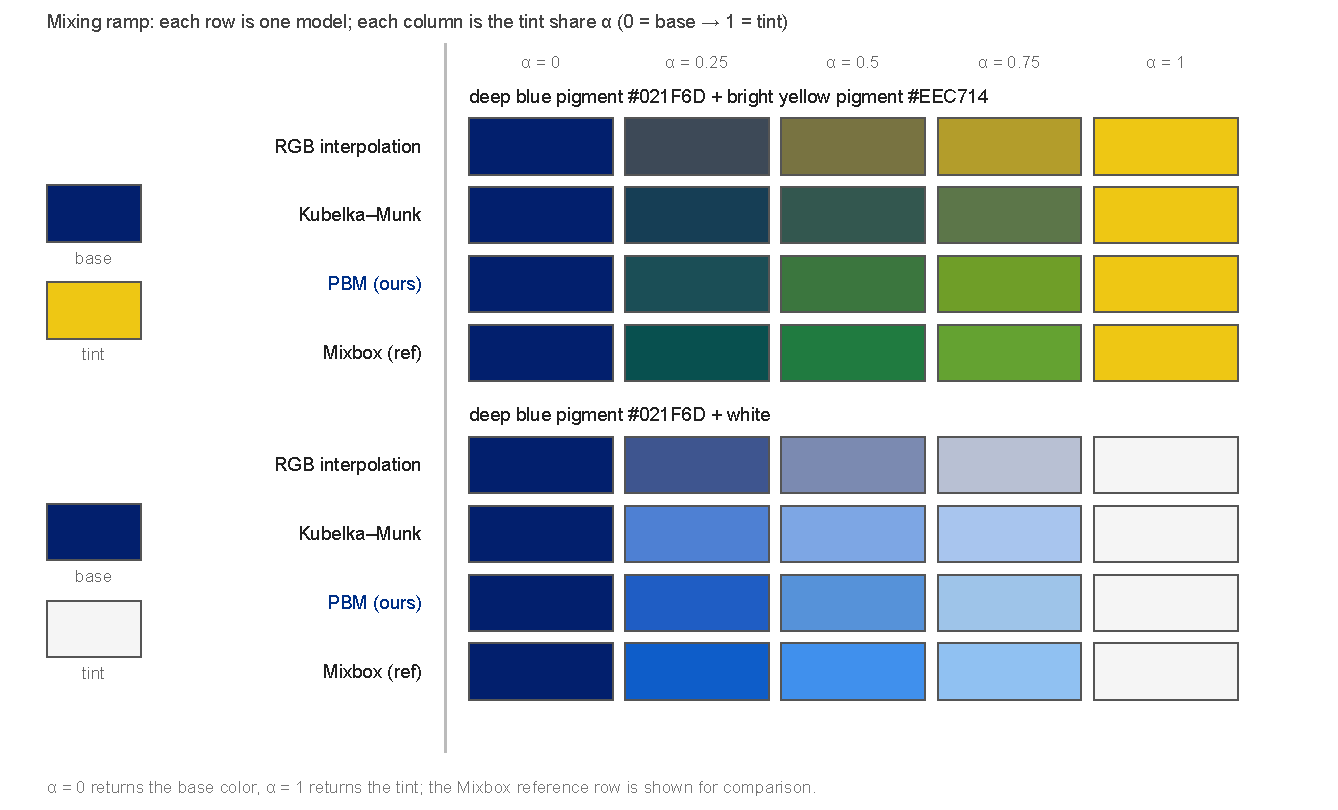
\includegraphics[width=\linewidth]{fig1-mixing.pdf}
\caption{Mixing behavior of RGB interpolation, spectral K--M, PBM, and the Mixbox reference. Top: a deep blue pigment mixed with a bright yellow pigment. Bottom: the same deep blue mixed with white. Each row is one model; each column is the tint share $\alpha$ ($\alpha=0$ returns the base color, $\alpha=1$ the tint). The K--M row is the synthetic spectral truth of \cref{sec:synthetic}: synthetic pigment spectra mixed by two-constant Duncan superposition, with the rendered colors of the pure pigments as inputs. PBM follows the same qualitative families (yellow $\times$ blue $\rightarrow$ green; deep $+$ white remains chromatic).}
\label{fig:overview}
\end{figure}

\section{Background and Related Work}
\label{sec:background}

\subsection{The Physics of Pigment Mixing}
\label{sec:km}

The color of a pigmented layer results from wavelength-selective absorption and scattering by pigment particles. In the two-flux Kubelka--Munk model, each pigment $i$ is described by an absorption coefficient $K_i(\lambda)$ and a scattering coefficient $S_i(\lambda)$. For non-negative concentrations $c_i$ summing to one, Duncan's superposition gives
\begin{equation}
K(\lambda)=\sum_i c_i K_i(\lambda),\qquad
S(\lambda)=\sum_i c_i S_i(\lambda),
\label{eq:duncan}
\end{equation}
and the reflectance of an opaque layer at wavelength $\lambda$ is
\begin{equation}
\Rinf(\lambda)=1+\kappa(\lambda)-\sqrt{\kappa(\lambda)^{2}+2\kappa(\lambda)},
\qquad \kappa(\lambda)=\frac{K(\lambda)}{S(\lambda)}.
\label{eq:km}
\end{equation}
A display color is obtained by integrating the reflectance against an illuminant and the CIE standard observer, optionally applying Saunderson's surface correction, and converting to sRGB \cite{saunderson1942,haase1992,wyszecki2000}. The model is physically interpretable but requires spectral data: an RGB triple does not determine $K_i(\lambda)$ or $S_i(\lambda)$, and mixing two arbitrary RGB colors requires solving for pigment concentrations numerically because \cref{eq:km} has no analytic inverse with respect to RGB.

\subsection{Related Work}
\label{sec:related}

\paragraph{RGB interpolation.}
Linear interpolation, to which blending, compositing, and smudging reduce in most pipelines, models additive light mixing. It is exact for light but produces gray from complementary pigments and desaturates dark colors toward white, the two defects that motivate this work.

\paragraph{RYB interpolation.}
Gossett and Chen \cite{gossett2004} interpolate eight hand-selected colors in a three-dimensional cube so that blue and yellow produce green. The construction reproduces the direction of the hue shift but not the colorimetric behavior of pigments; we do not evaluate it in this work.

\paragraph{Subtractive and hybrid models.}
Overlaid-filter models account for absorption but not scattering; yellow and blue produce green, but the result is too dark and off-hue. Hybrid subtractive--additive formulas \cite{simonot2014} lighten the result while retaining much of the color error.

\paragraph{Data-driven approaches.}
Lu et al. \cite{lu2014} interpolate example pigment mixtures at predetermined ratios. Pigment-palette extraction \cite{aharoni2017,tan2019} and reduced-order parametric models \cite{shugrina2020} target artwork manipulation rather than interactive mixing of arbitrary colors.

\paragraph{Mixbox.}
Mixbox \cite{sochorova2021} encodes an sRGB color into a seven-dimensional latent vector---four pigment concentrations (Phthalo Blue, Quinacridone Magenta, Hansa Yellow, Titanium White) and three additive residuals---trained on measured pigment spectra so that latent mixtures remain inside the sRGB gamut. Latents are mixed linearly and decoded with $256^{3}$ encoder and decoder tables. The model is the reference for the present work. It is trained and table-based rather than analytic, and the reference implementation is distributed under a non-commercial license.

\section{Model}
\label{sec:model}

\subsection{Notation and Composition}
\label{sec:notation}

PBM operates on sRGB display values in $[0,1]$; no linearization, transfer function, or color-space conversion is applied. The model is the composition of a mixing core and a repair layer,
\begin{equation}
\mathbf{o}=\clamp\bigl(\mathbf{C}+\mathbf{d},\,0,\,1\bigr),\qquad
\mathbf{C}=\operatorname{Core}(\cb,\ct,\alpha),\qquad
\mathbf{d}=\operatorname{Repair}(\cb,\ct,\alpha,\mathbf{C}),
\label{eq:composition}
\end{equation}
where $\cb$ is the base color, $\ct$ the tint, and $\alpha=\clamp(A,0,1)$ the tint share: $\alpha=0$ returns the base and $\alpha=1$ the tint.

\begin{figure}[t]
\centering
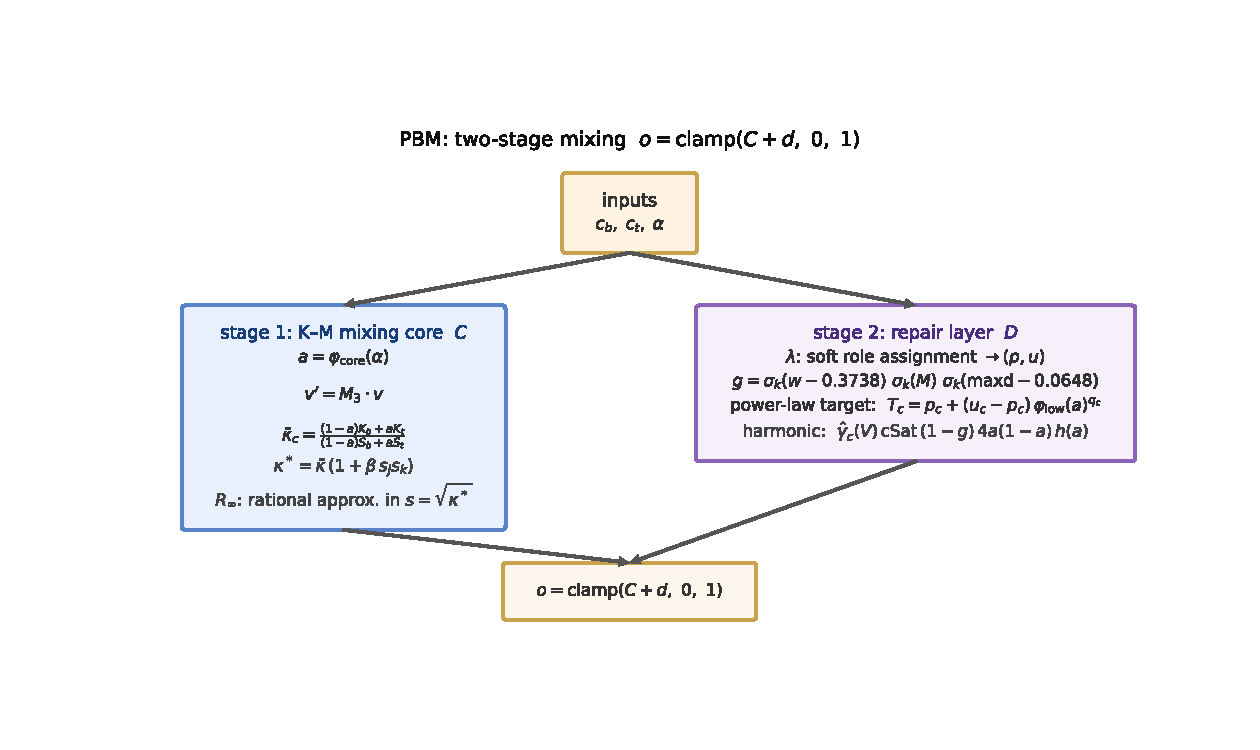
\includegraphics[width=0.82\linewidth]{fig2-architecture.pdf}
\caption{PBM data flow. Both inputs feed the K--M mixing core ($C$). The repair layer assigns the pigment and bright-end roles ($\lambda$), evaluates the per-channel power-law target ($T$) gated by $g$, and adds the harmonic correction ($\hat{\gamma}$). The correction $\mathbf{d}$ is added to the core output and clamped.}
\label{fig:architecture}
\end{figure}

The repair layer is asymmetric in the roles of its two arguments, whereas the core is symmetric. A soft role assignment blends the two role orderings so that the complete model is exchange-symmetric,
\begin{equation}
F(\cb,\ct,\alpha)\equiv F(\ct,\cb,1-\alpha),
\label{eq:symmetry}
\end{equation}
up to floating-point rounding.

We write $\vp$ for the pigment endpoint and $\vu$ for the bright endpoint, as selected by the role assignment (\cref{sec:role}): the input with the smaller maximum channel plays the pigment. From $\vp$ we define
\begin{equation}
M=\max(\vp),\qquad m=\min(\vp),\qquad \mathrm{maxd}=M-m,\qquad
w=\max\bigl(\min(\vp),\min(\vu)\bigr).
\label{eq:notation}
\end{equation}
The soft step with slope $k$ is $\sigmak(x)=\clamp(kx,0,1)$, and $\ssf(x;a,b)$ is the $C^{1}$ smoothstep on $[a,b]$.

\subsection{The Structural Limitation of Display-Value K/S Mixing}
\label{sec:defect}

The core mixes in display-value space using analytic defaults for absorption and scattering,
\begin{equation}
K(v)=\tfrac12(1-v)^{2},\qquad S(v)=\max(v,\varepsilon),\qquad \varepsilon=0.00157634.
\label{eq:ks-default}
\end{equation}
For a white input, $v=1$, hence $K=0$ and $S=1$, whereas a deep pigment has $S$ in the range $0.05$--$0.35$. At any $\alpha$, the scattering of white dominates the denominator of the concentration-weighted ratio, and the per-channel $\kappa$ values collapse toward each other.

As a single-channel illustration, ignore the cross-channel matrix and the mutual-absorption correction and consider the red channel of the deep blue $\#0D1B44=(0.051,0.106,0.267)$ mixed with white at $\alpha=0.5$:
\begin{equation}
\bar{\kappa}_{R}=
\frac{0.5\,K(0.051)+0.5\,K(1)}{0.5\,S(0.051)+0.5\,S(1)}
=\frac{0.5\times0.451}{0.5\times0.051+0.5\times1}=0.429,
\label{eq:defect}
\end{equation}
which gives $\Rinf\approx0.41$. The Mixbox reference reads $0.28$ for this channel. The absorbing channel is washed out. Conversely, the blue channel reads $0.89$ in the reference against $0.53$ in the single-channel computation; it is under-lightened. This imbalance is structural: the $S=1$ of white dominates the mixture denominator for every $\alpha$, and the weighted $K$ and $S$ are constrained by the same weights, so rescaling $K/S$ at the mixing stage cannot restore the absorbed channel. Raw display-value K--M superposition measures a mean $\Delta E_{00}$ of 10.30 on the dark-plus-white suite (\cref{tab:insample}).

\subsection{Stage 1: The K--M Mixing Core}
\label{sec:core}

Both inputs are transformed by a cross-channel matrix $\Mthree$ with row sums equal to one,
\begin{equation}
\mathbf{v}'=\Mthree\mathbf{v},\qquad
\Mthree=
\begin{pmatrix}
0.74523981 & 0.30403013 & -0.04926994\\
0 & 0.74093256 & 0.25906744\\
0 & 0 & 1
\end{pmatrix}.
\label{eq:m3}
\end{equation}
Absorption and scattering are evaluated with the analytic defaults of \cref{eq:ks-default}. The mixing ratio in each channel follows Duncan's concentration structure, clamped to $[10^{-6},10^{4}]$:
\begin{equation}
\bar{\kappa}_{c}=
\frac{(1-a)\,K(v'_{b,c})+a\,K(v'_{t,c})}
     {(1-a)\,S(v'_{b,c})+a\,S(v'_{t,c})},
\label{eq:kappa}
\end{equation}
where $a=\varphi_{\mathrm{core}}(\alpha)$ is the progress after endpoint compression.

A per-channel mutual-absorption correction uses the other two channels $\{j,k\}$:
\begin{equation}
s'_{c}=\frac{\sqrt{\bar{\kappa}_{c}}}{1+\sqrt{\bar{\kappa}_{c}}},\qquad
\kstar_{c}=\bar{\kappa}_{c}\bigl(1+\beta_{c}\,s'_{j}\,s'_{k}\bigr),\qquad
\beta=(-0.69372345,\,-0.48397409,\,-0.24977842).
\label{eq:beta}
\end{equation}
Because $s'\in[0,1)$ and $\beta_{c}<0$, the correction reduces $\kappa$ when the other channels are bright.

The reflectance is evaluated with a rational approximation in $s=\sqrt{\kstar}$,
\begin{equation}
\Rinf\approx\frac{1}{1+s\bigl(a_{1}+s(a_{2}+s\,a_{3})\bigr)},\qquad
(a_{1},a_{2},a_{3})=\Bigl(\sqrt{2},\,1,\,\tfrac{1}{2\sqrt{2}}\Bigr),
\label{eq:rational}
\end{equation}
which matches the first four Taylor coefficients of $\Rinf$ at $s=0$. Over the clamped range $\kstar\in[10^{-6},10^{4}]$, the maximum absolute error of \cref{eq:rational} is $8.1\times10^{-3}$ (at $\kstar\approx8.1$); for $\kstar\le1$ it is $2.5\times10^{-3}$. The output is mapped back and clamped:
\begin{equation}
\mathbf{C}=\clamp\bigl(\Mthree^{-1}\,\Rinf(\boldsymbol{\kstar}),\,0,\,1\bigr).
\label{eq:core-output}
\end{equation}

\paragraph{Dynamic progress.}
The reference converges faster than display-value $\kappa$ mixing as $\alpha\to1$. Inverting the reference at $\alpha=0.99$ indicates that the power-law target would require an equivalent progress of about $10^{-3}$ (\cref{sec:inversion}), i.e.\ that 99\% of the blend behaves like 99.9\%. We encode this with a symmetric endpoint-compression map applied to the core's mixing ratio,
\begin{equation}
\varphi_{\mathrm{low}}(x)=
\begin{cases}
x, & x\ge w_{\varphi},\\[2pt]
\bigl(1-\ssf(x;0,w_{\varphi})\bigr)x^{p_{\varphi}}+\ssf(x;0,w_{\varphi})\,x, & x<w_{\varphi},
\end{cases}
\label{eq:philow}
\end{equation}
\begin{equation}
\varphi_{\mathrm{core}}(x)=
\begin{cases}
\varphi_{\mathrm{low}}(x), & x<0.5,\\
1-\varphi_{\mathrm{low}}(1-x), & x\ge0.5,
\end{cases}
\label{eq:phicore}
\end{equation}
with $p_{\varphi}=1.96522814$ and $w_{\varphi}=0.08$. The map is $C^{1}$ and antisymmetric about $x=0.5$, so the core remains exchange-symmetric; $\varphi_{\mathrm{low}}(x)=x$ for $x\ge w_{\varphi}$, so only the tails are affected.

\subsection{Stage 2: The Repair Layer}
\label{sec:repair}

The repair layer computes a correction $\mathbf{d}$ to the core output. It consists of a role assignment, a gate, a per-channel power-law target, and an additive harmonic correction.

\paragraph{Soft role assignment.}
\label{sec:role}
The pigment endpoint is the input with the smaller maximum channel. A hard argmin would switch discontinuously when $\max(\cb)=\max(\ct)$, so we use a soft membership
\begin{equation}
\lambda=\ssf\!\left(\frac{\max(\ct)-\max(\cb)+E_{W}}{2E_{W}};\,0,\,1\right),
\qquad E_{W}=0.08.
\label{eq:lambda}
\end{equation}
$\lambda=1$ selects $(\vp,\vu,a)=(\cb,\ct,\alpha)$; $\lambda=0$ selects $(\ct,\cb,1-\alpha)$; inside the tie band $|\max(\ct)-\max(\cb)|<E_{W}$ the two branches are blended,
\begin{equation}
\mathbf{d}=\lambda\,D(\cb,\ct,\alpha)+(1-\lambda)\,D(\ct,\cb,1-\alpha).
\label{eq:dblend}
\end{equation}
Outside the band, $\lambda$ is exactly $0$ or $1$ and the layer reduces to one evaluation of $D$. For uniformly sampled sRGB pairs, the band contains approximately $26\%$ of pairs (measured $26.6\%$ on the T3 draw with seed 20260808 and $26.2\%$ on $2\times10^{5}$ uniform pairs); the branch is therefore skipped for about three quarters of random inputs. The role signal is the maximum channel; a luminance signal was also considered but changed the role decision for a non-negligible fraction of random pairs and was not adopted.

\paragraph{Dark-plus-light gate.}
The power-law target is applied only in the dark-pigment/light-end region. The gate is a product of three soft steps with the shared slope $k=11.0163945$:
\begin{equation}
g=\sigmak(w-0.37375181)\cdot\sigmak(M)\cdot\sigmak(\mathrm{maxd}-0.06479933).
\label{eq:gate}
\end{equation}
The first factor opens when the brighter endpoint is close to achromatic-bright ($w$ large); the second reduces the gate for near-black pigments ($M\lesssim1/k\approx0.09$); the third requires a minimum chroma range. Each transition has width $1/k\approx0.091$, so the gate introduces no hard cutoff. For light or nearly achromatic pigments, $g=0$ and the core output is used directly.

\paragraph{Power-law target.}
Within the gate region, the target follows a per-channel power law from the pigment toward the bright end:
\begin{equation}
T_{c}=p_{c}+(u_{c}-p_{c})\,\varphi_{\mathrm{low}}(a)^{q_{c}}.
\label{eq:target}
\end{equation}
The exponent $q_{c}$ controls how quickly channel $c$ brightens and is composed of four terms.

\emph{(a) Soft-step staircase.} Inverting the reference on anchored colors (\cref{sec:inversion}) shows that the required exponent decreases with the channel value $v$: dark segments hold absorption (high $q$), bright segments advance quickly (low $q$). The structure is represented by two steps,
\begin{equation}
q^{f}(v)=c_{1}^{f}+(c_{2}^{f}-c_{1}^{f})\,\sigmak(v-t_{1})+(c_{3}-c_{2}^{f})\,\sigmak(v-t_{2}),
\qquad f\in\{B,G\},
\label{eq:staircase}
\end{equation}
with $t_{1}=0.04350222$, $t_{2}=0.26436295$, and the coefficients in \cref{tab:softstep}. The red family is neutral, $q^{R}\equiv1$; its channel-dependent behavior is carried by the directional responses in (d).

\begin{table}[t]
\centering
\small
\caption{Soft-step coefficients of the brightening exponent (\cref{eq:staircase}).}
\label{tab:softstep}
\begin{tabular}{lcccc}
\toprule
Family & $c_{1}$ (dark) & $c_{2}$ (mid) & $c_{3}$ (bright) & Step positions / slope \\
\midrule
$B$ (blue, $B$ maximal) & 0.91483121 & 0.32538955 & 0.18785981 & $t_{1}=0.04350222$, $t_{2}=0.26436295$ \\
$G$ (green, $G$ maximal) & 0.57387051 & 0.596528 & 0.18785981 & $k=11.0163945$ (shared) \\
$R$ (red) & --- & --- & --- & $q^{R}\equiv1$ \\
\bottomrule
\end{tabular}
\end{table}

\emph{(b) Family soft mixing.} The family weights are pairwise dominance comparisons on the pigment channels,
\begin{equation}
g_{R}=\tfrac12\,\sigma_{8}(v_{R}-v_{G})+\tfrac12\,\sigma_{8}(v_{R}-v_{B}),
\qquad g_{G},,g_{B}\ \text{analogously},
\label{eq:family-weights}
\end{equation}
where $\sigma_{8}(x)=\clamp(8x,0,1)$. The base exponent is
\begin{equation}
q_{c}^{\mathrm{base}}=\frac{g_{B}q_{c}^{B}+g_{G}q_{c}^{G}+g_{R}q_{c}^{R}}{g_{R}+g_{G}+g_{B}}.
\label{eq:qbase}
\end{equation}
When $g_{R}+g_{G}+g_{B}<10^{-6}$, the base reduces to the equal-weight mean, which covers near-gray pigments.

\emph{(c) Channel residuals.} For near-zero channels, the reference curves depend on the channel rather than on the pigment. The residual is a shared amplitude times a smooth envelope,
\begin{equation}
q_{c}\mathrel{+}=\mathrm{RES}_{c}\,e(v_{c}),\qquad
e(v)=
\begin{cases}
A\bigl(1-v/W\bigr)^{2}, & v<W,\\
0, & v\ge W,
\end{cases}
\label{eq:residual}
\end{equation}
with $A=0.83421324$, $W=0.14196781$, and $\mathrm{RES}=(0,\,-0.24164942,\,-0.24164942)$; the red residual is zero. Unlike a piecewise-linear envelope, \cref{eq:residual} is $C^{1}$ at $v=W$ and needs three constants instead of eight.

\emph{(d) Channel coupling and directional responses.} Colors with two high channels brighten more slowly, and each family carries a linear directional response in the pigment channels:
\begin{equation}
q_{c}\mathrel{+}=0.42818849\,\sigma_{4.13539205}\Bigl(\max_{i\ne c}v_{i}\Bigr),
\label{eq:coupling}
\end{equation}
\begin{equation}
q_{c}\mathrel{+}=g_{R}\,g^{\mathrm{RTH}}\,\delta^{R}_{c}+g_{B}\,\delta^{B}_{c}+g_{G}\,\delta^{G}_{c},
\qquad
g^{\mathrm{RTH}}=\sigma_{8}(v_{R}-0.21929798),
\label{eq:directional}
\end{equation}
with
\begin{align}
\delta^{R}&=\bigl[-0.28030789-0.31011215\,v_{R},\nonumber\\
&\qquad 0.33194666-1.19791733\,v_{G},\; -0.45218018+1.71390058\,v_{G}\bigr],\nonumber\\
\delta^{B}&=\bigl[0.40713961,\; -0.08390816+0.76274462\,v_{G},\; 0\bigr],\label{eq:deltas}\\
\delta^{G}&=\bigl[-0.2367074+0.72220875\,v_{R},\; 0,\; -0.30067864+1.03098891\,v_{G}\bigr].\nonumber
\end{align}
The range gate $g^{\mathrm{RTH}}$ is necessary: the linear expressions change sign below $v_{R}=0.21929798$. For the two near-black reds $\#280501$ and $\#250903$ over $\alpha\in[0.1,0.9]$, disabling the gate raises the mean $\Delta E_{00}$ from 2.80 to 15.76 (maximum from 4.14 to 19.04).

\paragraph{Harmonic correction.}
Inverting the reference on complementary pairs (\cref{sec:inversion}) reveals a residual concentrated in the middle of the mixing range with the shape $4a(1-a)$ and an amplitude that varies smoothly with the input colors. The correction is a linear model over a ratio-based feature template, attenuated at both endpoints:
\begin{equation}
d_{c}\mathrel{+}=\hat{\gamma}_{c}(\vp,\vu)\;\mathrm{cSat}(\vp,\vu)\;(1-g)\;4a(1-a)\;h(a),
\label{eq:harmonic}
\end{equation}
where
\begin{equation}
\begin{aligned}
h(a)&=\sigma_{14}(0.845-a),\\
\mathrm{cSat}(\vp,\vu)&=\ssf\bigl(\max(\vp)-\min(\vp);0.02,0.15\bigr)\\
&\qquad\cdot\ssf\bigl(\max(\vu)-\min(\vu);0.08,0.30\bigr).
\end{aligned}
\label{eq:csat}
\end{equation}
The factor $(1-g)$ excludes the dark-plus-light region. The chroma attenuation $\mathrm{cSat}$ drives the correction to zero when either endpoint approaches the achromatic axis. This attenuation is important for continuity: the ratio features have large gradients near zero chroma, and without $\mathrm{cSat}$ the maximum single-step output change under an 8-bit input perturbation rises from 1.39 to 2.53 $\Delta E_{00}$ (\cref{sec:continuity}).

The amplitude is a linear function of a seventeen-feature template $V$ computed once per pair,
\begin{equation}
\hat{\gamma}_{c}(\vp,\vu)=w_{0}^{c}+\sum_{j}w_{j}^{c}\,V_{j},
\label{eq:gamma}
\end{equation}
with $17$ coefficients per channel ($51$ in total), fitted by least squares on a corpus of complementary-family and random measurements (\cref{sec:estimation}). Every feature is a polynomial, a ratio of channel differences, or a clamped linear form: the template contains no trigonometric function, so the harmonic correction costs only multiplications, additions, and one division per ratio. The template is defined in \cref{tab:features}; the coefficients are listed in \cref{app:coeff}. Unlike a learned latent representation, the template is hand-designed from the inversion measurements, and no data are stored at runtime.

\begin{table}[t]
\centering
\scriptsize
\setlength{\tabcolsep}{3pt}
\caption{The harmonic feature template (seventeen features including the intercept, used by all three channels). All features are computed once per pair from the pigment endpoint $\vp$ and the bright endpoint $\vu$.}
\label{tab:features}
\begin{tabular}{ll}
\toprule
Feature & Definition \\
\midrule
intercept & $1$ \\
\texttt{lum} & $0.2126\,p_{R}+0.7152\,p_{G}+0.0722\,p_{B}$ \\
\texttt{lumU} & $0.2126\,u_{R}+0.7152\,u_{G}+0.0722\,u_{B}$ \\
\texttt{pm}, \texttt{pn} & $\max(\vp)$, $\min(\vp)$ \\
\texttt{Mmn} & $\max(\vp)\cdot\min(\vp)$ \\
\texttt{span} & $(\max(\vp)-\min(\vp))(\max(\vu)-\min(\vu))$ \\
\texttt{op} & $1-\tfrac12\bigl[(\max(\vp)-\min(\vp))+(\max(\vu)-\min(\vu))\bigr]$ \\
\texttt{u2} & $u_{B}$ \\
\texttt{dcAbs} & $|u_{R}-p_{R}|$ \\
\texttt{wUcP} & $(u_{R}-u_{B})(p_{B}-p_{R})$ \\
\texttt{dg}, \texttt{ur} & $d_{g}=(p_{G}-p_{B})/\max(M-m,\epsilon)$,\quad $u_{r}=(u_{R}-u_{B})/\max(u_{\max}-u_{\min},\epsilon)$ \\
\texttt{drur}, \texttt{dgug} & $d_{r}u_{r}$, $d_{g}u_{g}$, with $d_{r}=(p_{R}-p_{B})/\cdots$ and $u_{g}=(u_{G}-u_{B})/\cdots$ \\
\texttt{dcmucm} & $d_{cm}u_{cm}$, with $d_{cm}=(p_{R}-p_{G})/\cdots$ and $u_{cm}=(u_{R}-u_{G})/\cdots$ \\
\texttt{gRu} & $\tfrac12\sigma_{8}(u_{R}-u_{G})+\tfrac12\sigma_{8}(u_{R}-u_{B})$ \\
\bottomrule
\end{tabular}
\end{table}

\subsection{Algorithm and Boundary Behavior}
\label{sec:algorithm}

The complete procedure is given in \cref{alg:pbm}. The endpoint-copy step makes $\alpha=0$ and $\alpha=1$ exact by construction. All remaining operations are compositions of continuous functions---clamps, powers, smoothsteps, and linear forms---so the model is continuous; no branch changes the value of an output discontinuously. \Cref{tab:boundary} summarizes the boundary properties and the measured values.

Here $\operatorname{Core}$ denotes the composition of \cref{eq:phicore,eq:m3,eq:kappa,eq:beta,eq:core-output}, and $D$ denotes the repair branch of \cref{eq:gate,eq:target,eq:harmonic}.

\begin{algorithm}[t]
\caption{PBM mixing.}
\label{alg:pbm}
\KwIn{base $\cb$, tint $\ct$ (sRGB display values in $[0,1]$), ratio $A$}
\KwOut{mixed color $\mathbf{o}$}
$\alpha\gets\clamp(A,0,1)$\;
\If{$\alpha=0$}{\Return{$\cb$}}
\If{$\alpha=1$}{\Return{$\ct$}}
$\mathbf{C}\gets\operatorname{Core}(\cb,\ct,\alpha)$\;
$t_{e}\gets\clamp\bigl((\max(\ct)-\max(\cb)+E_{W})/(2E_{W}),0,1\bigr)$\;
\uIf{$t_{e}\le0$}{$\mathbf{d}\gets D(\ct,\cb,1-\alpha,\mathbf{C})$}
\uElseIf{$t_{e}\ge1$}{$\mathbf{d}\gets D(\cb,\ct,\alpha,\mathbf{C})$}
\Else{$\lambda\gets\ssf(t_{e})$;\; $\mathbf{d}\gets\lambda D(\cb,\ct,\alpha,\mathbf{C})+(1-\lambda)D(\ct,\cb,1-\alpha,\mathbf{C})$}
\Return{$\clamp(\mathbf{C}+\mathbf{d},0,1)$}\;
\end{algorithm}

\begin{table}[t]
\centering
\small
\caption{Boundary behavior of PBM.}
\label{tab:boundary}
\begin{tabular}{p{0.28\linewidth}p{0.64\linewidth}}
\toprule
Property & Guarantee \\
\midrule
$\alpha=0,1$ & returns the inputs exactly (T4 maximum channel error 0.00000). \\
Outside the gate & $g=0$: core output plus the harmonic correction; inside: power-law target plus harmonic correction; the transition is continuous. \\
Continuity & composition of continuous functions; measured maximum single-step $\Delta E_{00}$ of 1.388 under an 8-bit perturbation, with zero exceedances of 1.53. \\
Exchange symmetry & $F(\cb,\ct,\alpha)\equiv F(\ct,\cb,1-\alpha)$; maximum observed RGB difference $6.7\times10^{-16}$ over 5000 random pairs (seed 20260808). \\
\bottomrule
\end{tabular}
\end{table}

\paragraph{Complexity and implementation.}
The model performs a fixed number of arithmetic operations: two matrix-vector products for the inputs, one for the output, six square roots, up to five powers, and no trigonometric or logarithmic evaluation. It has no loops over data, no tables, and no iteration; its time and space complexity is $O(1)$. A reference implementation is available in four languages (JavaScript, Python, Java, and C++) with identical constants; a cross-language test over 2000 random pairs measures a maximum RGB channel difference of $5\times10^{-10}$, which is consistent with the nine-decimal serialization used by the test and with library-level differences in the elementary functions.

The constants of the model are frozen in the implementation. Changing them requires re-running the estimation and the cross-language consistency test; the four ports are kept identical at the level of numeric literals.

\section{Parameter Estimation}
\label{sec:estimation}

\subsection{Reference and Metric}
\label{sec:reference}

All constants are fitted to, or inverted from, output measurements of the public Mixbox~2.0 API \texttt{lerpFloat}, using the sRGB display-value float path. The reference is loaded from the official distribution for research comparison only. The metric is CIEDE2000 \cite{sharma2005} with $k_{L}=k_{C}=k_{H}=1$, validated against the 34 reference pairs of Sharma et al.\ (maximum absolute deviation $4.95\times10^{-5}$). Mixing is performed on display values without linearization; $\Delta E_{00}$ is computed after conversion to CIELAB under D65.

\subsection{Inversion Measurements}
\label{sec:inversion}

The design is driven by measurements that invert the reference rather than by assumptions about pigment physics. For each anchored color pair, the per-channel exponent required by a power-law trajectory is read from the reference output at progress $\alpha$:
\begin{equation}
p_{c}(\alpha)=\frac{\ln\bigl((r_{c}-v_{c})/(1-v_{c})\bigr)}{\ln\alpha},
\label{eq:inversion}
\end{equation}
where $v_{c}$ is the pigment channel value and $r_{c}$ the reference output.

Three structural observations follow (\cref{app:inversion} reports the supporting tables). First, the inverted exponent is approximately constant in $\alpha$: it drifts by less than 0.2 over $\alpha\in[0.1,0.9]$ in every family, which supports a single-exponent model; the drift near $\alpha\to1$ is the region addressed by the $\varphi$ map. Second, the exponent decreases with the channel value in a two-step pattern---dark segments hold absorption, bright segments advance quickly---which is the empirical basis of \cref{eq:staircase}. Third, the residual structure is family- and channel-dependent: near-zero channels depend on the channel rather than on the pigment, red-family pigments hold their green absorption when brightened, and complementary mixtures leave a residual of approximate shape $4a(1-a)$ in the middle of the range. These observations motivate the residual, coupling, directional, and harmonic terms of \cref{sec:repair}.

\Cref{fig:staircase} plots the inverted exponents at $\alpha=0.5$ together with the soft-step approximations and the end-to-end inversion of the PBM output.

\begin{figure}[t]
\centering
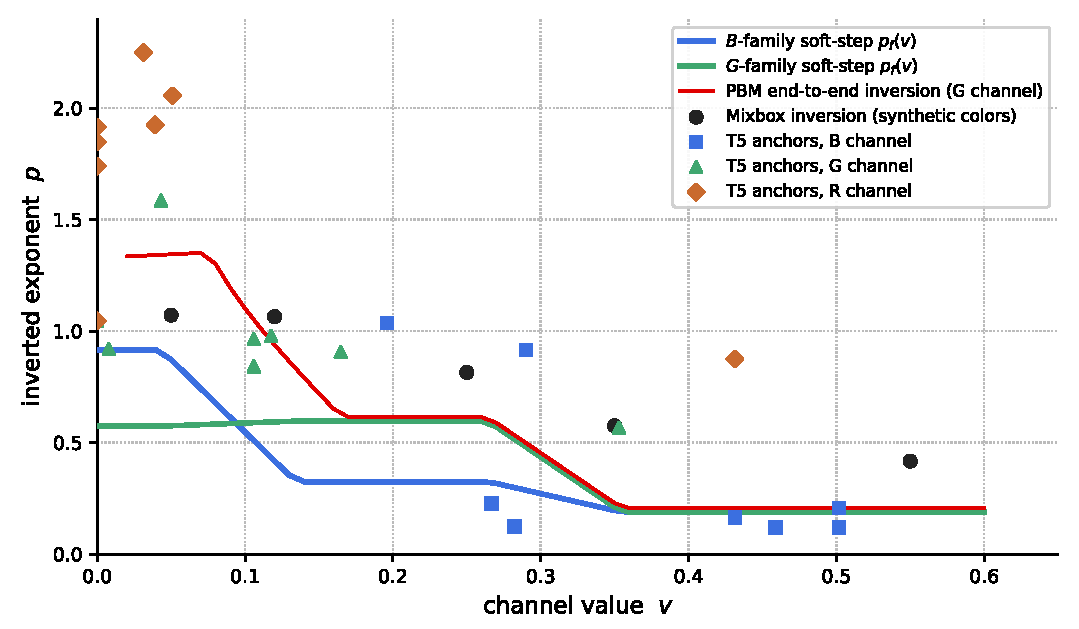
\includegraphics[width=0.78\linewidth]{fig3-staircase.pdf}
\caption{Inverted exponent $p$ at $\alpha=0.5$ as a function of the channel value $v$. Points: Mixbox inversion for synthetic colors and T5 anchors. Lines: the $B$- and $G$-family soft-step approximations and the end-to-end inversion of the PBM output (G channel).}
\label{fig:staircase}
\end{figure}

\subsection{Fitting Procedure}
\label{sec:fitting}

The estimation is two-stage and fully reproducible from the repository tooling.

\paragraph{Corpus.}
The fitting corpus contains the palette suite (T1), the stress-pair suite (T2), the first 800 random pairs of the T3 draw (seed 20260808), the dark-plus-white suite (T5), the two-sided tail suite (T5E), 6000 pseudo-random sRGB pairs (seed 999), and twelve anchored complementary pairs sampled at nineteen ratios; the anchored pairs carry a weight of ten so that the harmonic correction is fitted where it acts.

\paragraph{Harmonic coefficients.}
Because $\hat{\gamma}$ enters \cref{eq:harmonic} linearly, the 51 coefficients are obtained in closed form. For each corpus entry the two role branches contribute
\begin{equation}
\mathbf{y}=
\mathbf{r}-\mathbf{C}-\sum_{b}\lambda_{b}\,g_{b}\,(T_{b}-\mathbf{C}),
\qquad
\mathbf{A}=\sum_{b}\lambda_{b}\,g_{b}\,V_{b},
\label{eq:design}
\end{equation}
where $\mathbf{r}$ is the reference output and the sum runs over the one or two active branches; the coefficients solve the linear least-squares problem $\mathbf{A}\mathbf{w}\approx\mathbf{y}$ per channel, with a ridge of $10^{-6}$. Entries whose total gain $\sum_{b}\lambda_{b}g_{b}$ is below 0.02 are excluded, which leaves 4664 design rows.

\paragraph{Scalars.}
The remaining fourteen scalars---the two staircase positions, the three $B$-family levels and the shared upper level, the coupling amplitude and slope, the gate threshold, slope, and chroma-range threshold, the two envelope constants, the endpoint-compression exponent, and the residual amplitude---are refined by coordinate descent on the in-sample loss
\begin{equation}
L=\overline{\Delta E_{00}}+0.02\,\max\Delta E_{00}+\frac{1}{12}\cdot\overline{\Delta E_{00}}\big|_{\text{anchors}},
\label{eq:loss}
\end{equation}
where the first two terms are evaluated over T1, T2, the 800 fitting pairs of T3, and T5. One alternation is performed: the harmonic coefficients are re-fitted on the updated core, and the change is below 0.014 $\Delta E_{00}$ on every suite, i.e.\ the two stages have reached a fixed point. The fitted constants were then re-evaluated on held-out draws that were not used in fitting (\cref{sec:results}).

\paragraph{Structural simplifications adopted on measured evidence.}
The staircase slope is merged into the shared gate slope; the $G$ and $B$ upper staircase levels share one value; the $\varphi$ width shares $E_{W}=0.08$; the role signal is the maximum channel; and the residual envelope is the $C^{1}$ quadratic of \cref{eq:residual} rather than a piecewise-linear interpolation.

\subsection{Gate Sensitivity}
\label{sec:sensitivity}

To test whether the gate thresholds are tuned to a narrow optimum, each gate threshold and the shared slope $k$ were perturbed by $\pm10\%$ and $\pm20\%$ while all other parameters remained fixed (\cref{tab:sensitivity}). The mean $\Delta E_{00}$ changes by at most 0.11 on T5 and 0.05 on T3. The T5 mean is flat under $w_{0}$ and $\mathrm{maxd}_{0}$ perturbations and moves by at most 0.11 when $k$ is scaled; the T3 maximum grows from 19.4 to 25.2 at $w_{0}\times0.8$, because a small number of complementary pairs are sensitive to the gate boundary. The thresholds therefore sit on a plateau of the loss rather than at a knife edge.

\begin{table}[t]
\centering
\small
\caption{Gate-parameter sensitivity: change in mean $\Delta E_{00}$ ($\Delta$T5 / $\Delta$T3) under $\pm10\%$ and $\pm20\%$ perturbation of each fitted gate parameter, with all other parameters fixed.}
\label{tab:sensitivity}
\begin{tabular}{lcccc}
\toprule
Parameter & $\times0.8$ & $\times0.9$ & $\times1.1$ & $\times1.2$ \\
\midrule
$w_{0}$ (0.37375181) & $+0.000/-0.045$ & $+0.000/-0.023$ & $+0.000/+0.026$ & $+0.000/+0.081$ \\
$\mathrm{maxd}_{0}$ (0.06479933) & $-0.011/-0.003$ & $-0.007/-0.002$ & $+0.010/+0.002$ & $+0.025/+0.005$ \\
shared slope $k$ (11.0163945) & $+0.105/-0.001$ & $+0.029/-0.001$ & $+0.013/+0.002$ & $+0.038/+0.005$ \\
\bottomrule
\end{tabular}
\end{table}

\section{Evaluation}
\label{sec:evaluation}

\subsection{Protocol}
\label{sec:protocol}

The reference is Mixbox~2.0 \texttt{lerpFloat} on the sRGB display-value float path. The metric is CIEDE2000 with $k_{L}=k_{C}=k_{H}=1$, validated as described in \cref{sec:reference}. Random-set means are reported with bootstrap 95\% confidence intervals (1000 resamples, fixed resampling stream so that the reported intervals are reproducible). The perceptual scale of $\Delta E_{00}$ is used only qualitatively: below 1 is near the threshold of detection, 1--2 is visible on close inspection, 2--4 is clearly visible, and above 4 is a substantial difference.

The design targets for the repair layer are a mean $\Delta E_{00}$ below 5 and a maximum not exceeding 15 on the dark-plus-white suites. The main suites (T1--T3) are not designed to meet the maximum target, because pairs with a large lightness gap and hue opposition dominate their maxima; we report the maxima without treating them as acceptance criteria.

\subsection{Test Sets and Split}
\label{sec:sets}

\Cref{tab:sets} summarizes the test sets; \cref{app:suite} gives their exact construction, colors, $\alpha$ grids, and seeds.

\begin{table}[t]
\centering
\footnotesize
\setlength{\tabcolsep}{3pt}
\caption{Evaluation test sets.}
\label{tab:sets}
\begin{tabular}{p{0.16\linewidth}p{0.46\linewidth}rr}
\toprule
Set & Content & $n$ & Role \\
\midrule
T1 palette & all pairs of the preset palette ($10$ bases $\times$ $8$ tints) $\times$ $\alpha\in\{0.25,0.5,0.75\}$ & 240 & in-sample \\
T2 stress pairs & complementary 3, RYB mismatch 6, white/black 6, similar 4, each $\times$ 3 $\alpha$ & 57 & in-sample \\
T3 random & uniform sRGB pairs $\times$ $\alpha\in[0,1]$, fixed seed & 2000 & mixed \\
T4 identity & 10 colors $\times$ $\alpha\in\{0,1\}$ self-mixing & 20 & structural \\
T5 dark + white & 20 fixed deep colors $+$ 24 random $\times$ 9 $\alpha$ levels & 396 & in-sample \\
T5-heldout & random deep colors (fresh seed 20260812) $\times$ 9 $\alpha$ levels & 216 & held-out \\
tail & T5 fixed colors $\times$ $\alpha\in[0.92,0.99]$ $+$ blind-spot colors $\times$ full $\alpha$ & 241 & in-sample \\
T5E two-sided tail & chromatic deep colors $\times$ deep-side $\alpha$ $+$ near-neutral deep colors $\times$ both sides & 240 & in-sample \\
\bottomrule
\end{tabular}
\end{table}

The fitting corpus contains T1, T2, T5, T5E, the tail set, and the first 800 pairs of T3 (seed 20260808). Held-out data are the disjoint T3 slice $[800,2000)$, two independent T3 draws (seeds 20260809 and 20260811, disjoint from every fitting seed), and T5-heldout (fresh seed 20260812). T3 uses a deterministic PRNG (mulberry32), so all draws are reproducible.

T5E covers the two tails that the other suites leave sparse: $\alpha\in\{0.001,\dots,0.1\}$ for 20 chromatic deep colors and 12 near-neutral deep colors, and $\alpha\in\{0.92,\dots,0.99\}$ for the same near-neutral colors. The near-neutral group has a chroma range below the gate threshold and is therefore mixed by the core alone; T5E supervises the $\varphi$ map in that region.

\subsection{Results}
\label{sec:results}

\Cref{tab:insample} reports in-sample results and \cref{tab:heldout} held-out results; \cref{fig:errhist} shows the error distributions.

\begin{table}[t]
\centering
\footnotesize
\setlength{\tabcolsep}{3pt}
\caption{In-sample results against Mixbox~2.0 ($\Delta E_{00}$ mean / max). T3(fit) is the first 800 pairs of the seed-20260808 draw.}
\label{tab:insample}
\begin{tabular}{lcccccc}
\toprule
Model & T1 & T2 & T3(fit) & T5 & tail & T4 \\
\midrule
PBM & \textbf{3.286 / 15.0} & \textbf{2.667 / 10.7} & \textbf{2.759 / 15.5} & \textbf{2.258 / 7.3} & \textbf{1.678 / 8.0} & 0.00000 \\
RGB interpolation & 5.053 / 39.0 & 5.526 / 39.4 & 3.374 / 27.5 & 8.127 / 20.9 & 5.878 / 20.6 & pass \\
K--M (display-value) & 4.867 / 27.4 & 5.199 / 25.2 & 3.964 / 23.7 & 10.299 / 23.6 & 9.877 / 24.1 & pass \\
\bottomrule
\end{tabular}
\end{table}

\begin{table}[t]
\centering
\footnotesize
\setlength{\tabcolsep}{3pt}
\caption{Held-out results against Mixbox~2.0 ($\Delta E_{00}$ mean / max; bootstrap 95\% CI for the PBM mean in the note).}
\label{tab:heldout}
\begin{tabular}{lcccc}
\toprule
Model & T3 slice $[800,2000)$ & T3 seed 09 & T3 seed 11 & T5-heldout \\
\midrule
PBM & \textbf{2.789 / 19.4} & \textbf{2.719 / 23.8} & \textbf{2.852 / 22.2} & \textbf{2.377 / 9.9} \\
RGB interpolation & 3.456 / 36.8 & 3.273 / 34.5 & 3.425 / 34.6 & 7.612 / 17.1 \\
K--M (display-value) & 4.002 / 31.5 & 3.918 / 31.4 & 4.010 / 32.8 & 9.517 / 17.3 \\
\bottomrule
\end{tabular}

\smallskip
{\scriptsize Bootstrap 95\% CI (mean), PBM: slice [2.662, 2.930]; seed 09 [2.612, 2.834]; seed 11 [2.742, 2.974]; T5-heldout [2.237, 2.540].}
\end{table}

\begin{figure}[t]
\centering
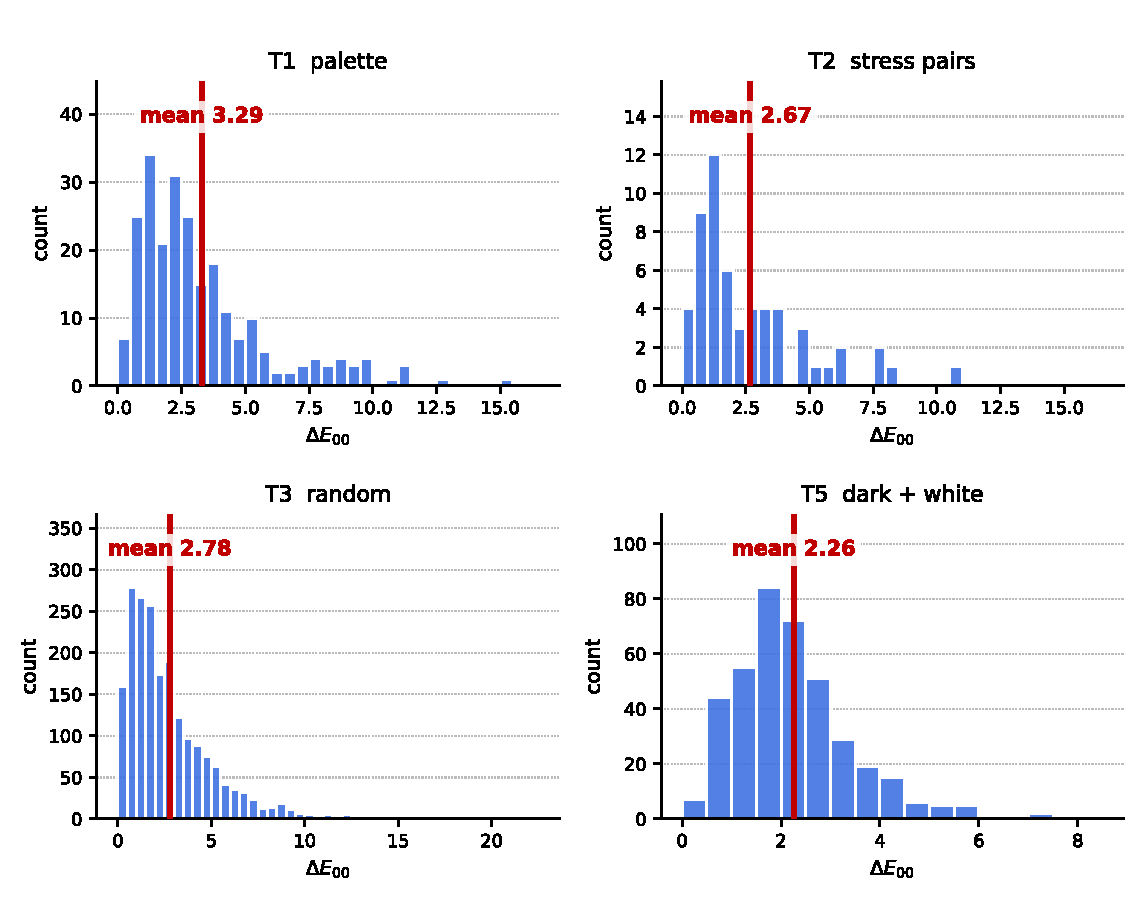
\includegraphics[width=0.72\linewidth]{fig4-error-dist.pdf}
\caption{$\Delta E_{00}$ histograms of PBM against Mixbox~2.0 on T1, T2, T3 (seed 20260808, $n=2000$), and T5 (bin width 0.5; red line: mean).}
\label{fig:errhist}
\end{figure}

Three observations follow. First, the held-out means differ from the fitting draw by at most 0.09 $\Delta E_{00}$ (T3 slice 2.789 versus 2.759), and the independent draws (2.719 and 2.852) lie in the same band. We find no evidence of overfitting under this protocol. Second, the held-out maxima (19.4--23.8) occur in random pairs that combine a large lightness gap with hue opposition; that family is the dominant source of large errors (\cref{sec:errors}). Third, the dark-plus-white repair generalizes: T5-heldout measures 2.377, 0.12 above the in-sample T5 mean, whereas RGB interpolation (7.61) and raw K--M (9.52) remain at their in-sample levels.

On T5E (240 samples), PBM measures a mean of 2.441, a maximum of 9.5, and a 95th percentile of 8.08, inside the design targets. Both applications of the $\varphi$ map improve the pairs they target: disabling the core map raises the T5E mean from 2.441 to 2.872, and disabling the map in the power-law target raises it to 2.881.

\subsection{Ablation}
\label{sec:ablation}

\Cref{tab:ablation} disables each component in the reference implementation. All variants are generated by textual patching of the algorithm source and verified to change the executed code; the tooling fails if a patch target is not found.

\begin{table}[t]
\centering
\footnotesize
\setlength{\tabcolsep}{2.5pt}
\caption{Ablation study ($\Delta E_{00}$ mean / max). T3 is the full seed-20260808 draw ($n=2000$).}
\label{tab:ablation}
\begin{tabular}{lccccc}
\toprule
Configuration & T1 & T2 & T3 & T5 & tail \\
\midrule
PBM (full) & \textbf{3.286 / 15.0} & \textbf{2.667 / 10.7} & \textbf{2.777 / 19.4} & \textbf{2.258 / 7.3} & \textbf{1.678 / 8.0} \\
$-$ cross-channel matrix $\Mthree$ & 3.674 / 23.8 & 3.534 / 14.9 & 3.218 / 25.6 & 2.259 / 7.3 & 1.678 / 8.0 \\
$-$ mutual absorption $\beta$ & 3.409 / 12.9 & 2.603 / 10.2 & 2.904 / 19.4 & 2.262 / 7.3 & 1.678 / 8.0 \\
$-$ channel coupling & 3.797 / 15.0 & 2.978 / 10.7 & 3.857 / 30.9 & 8.834 / 19.7 & 4.670 / 19.7 \\
$-$ directional responses & 3.491 / 15.0 & 2.741 / 10.7 & 2.969 / 24.2 & 4.739 / 15.2 & 3.429 / 12.4 \\
$-$ harmonic correction ($\hat{\gamma}$) & 3.649 / 15.3 & 3.543 / 13.5 & 2.890 / 20.0 & 2.258 / 7.3 & 1.678 / 8.0 \\
$-$ power-law repair ($g\equiv0$) & 3.700 / 15.0 & 3.091 / 10.7 & 3.248 / 20.4 & 9.823 / 23.8 & 8.448 / 24.0 \\
power-law everywhere ($g\equiv1$) & 4.785 / 25.2 & 5.237 / 24.4 & 2.967 / 26.1 & 2.248 / 7.3 & 1.654 / 8.0 \\
\bottomrule
\end{tabular}
\end{table}

The power-law repair and the channel coupling remain the two largest contributors on the dark-plus-white suite: T5 rises from 2.258 to 9.823 without the repair and to 8.834 without coupling. Coupling is also the strongest single term on the main suites (T3 2.777 to 3.857). The cross-channel matrix is second strongest on the main suites (T1 3.286 to 3.674; T2 2.667 to 3.534) and neutral on T5, where the repair dominates. Directional responses matter on T5 (4.739) and at the tail (3.429). Mutual absorption has a small, mixed effect: T2 improves without it (2.603) while T1 degrades (3.409), so it is retained. The harmonic correction improves all three main suites (T1 3.649 to 3.286; T2 3.543 to 2.667; T3 2.890 to 2.777) and is now a monotonically beneficial component. Forcing the power-law target everywhere degrades the main suites (T1 4.785, T2 5.237), so the gate's region selection is necessary.

\subsection{Error Structure}
\label{sec:errors}

The largest errors concentrate in pairs that combine a large lightness gap with hue opposition. The T1 worst pair is near-black $\#141417$ with orange $\#FF7A2A$ at $\alpha=0.25$ ($\Delta E_{00}=15.02$); the T2 worst pair is yellow $\#FFD61A$ with ultramarine $\#2E5EFF$ at $\alpha=0.75$ (10.70); the T3 worst pair is pale green-gray $\#C8D098$ with blue-violet $\#3A45E6$ at $\alpha\approx0.32$ (19.43). These are mixtures in which the reference's seven-dimensional latent space produces cross-channel correlations that a per-channel independent form cannot represent. Over $\alpha\in[0.05,0.95]$, the eight anchor pairs measure mean $\Delta E_{00}$ 2.85 (yellow $\times$ deep blue $\#FFC400+\#000F3D$), 3.16 (yellow $\times$ near-boundary $\#FFC400+\#000724$), 5.20 (red $\times$ green $\#A30000+\#00B359$), 7.04 (red $\times$ cyan $\#A30000+\#00D5C0$), 1.79 (magenta $\times$ green $\#E33BA8+\#00B359$), 3.80 (orange $\times$ blue $\#FF7A1A+\#2E5EFF$), 9.73 (orange $\times$ deep blue $\#FF7A1A+\#001B75$), and 5.07 (red $\times$ deep blue $\#A30000+\#001B75$), compared with a substantially larger error when the harmonic correction is removed (\cref{tab:ablation}).

On T5, the worst fixed-color pair is the dark violet $\#080248$ mixed with white at $\alpha=0.4$ ($\Delta E_{00}=7.3$); among the random deep colors the worst case is 7.3 as well. The two near-black reds in T5 ($\#280501$ and $\#250903$) measure a mean of 2.80 and a maximum of 4.14 over $\alpha\in[0.1,0.9]$ with the range gate; disabling the gate raises these values to 15.76 and 19.04. \Cref{fig:white,fig:worst} show the deep-plus-white trajectories and the worst pairs.

\begin{figure}[t]
\centering
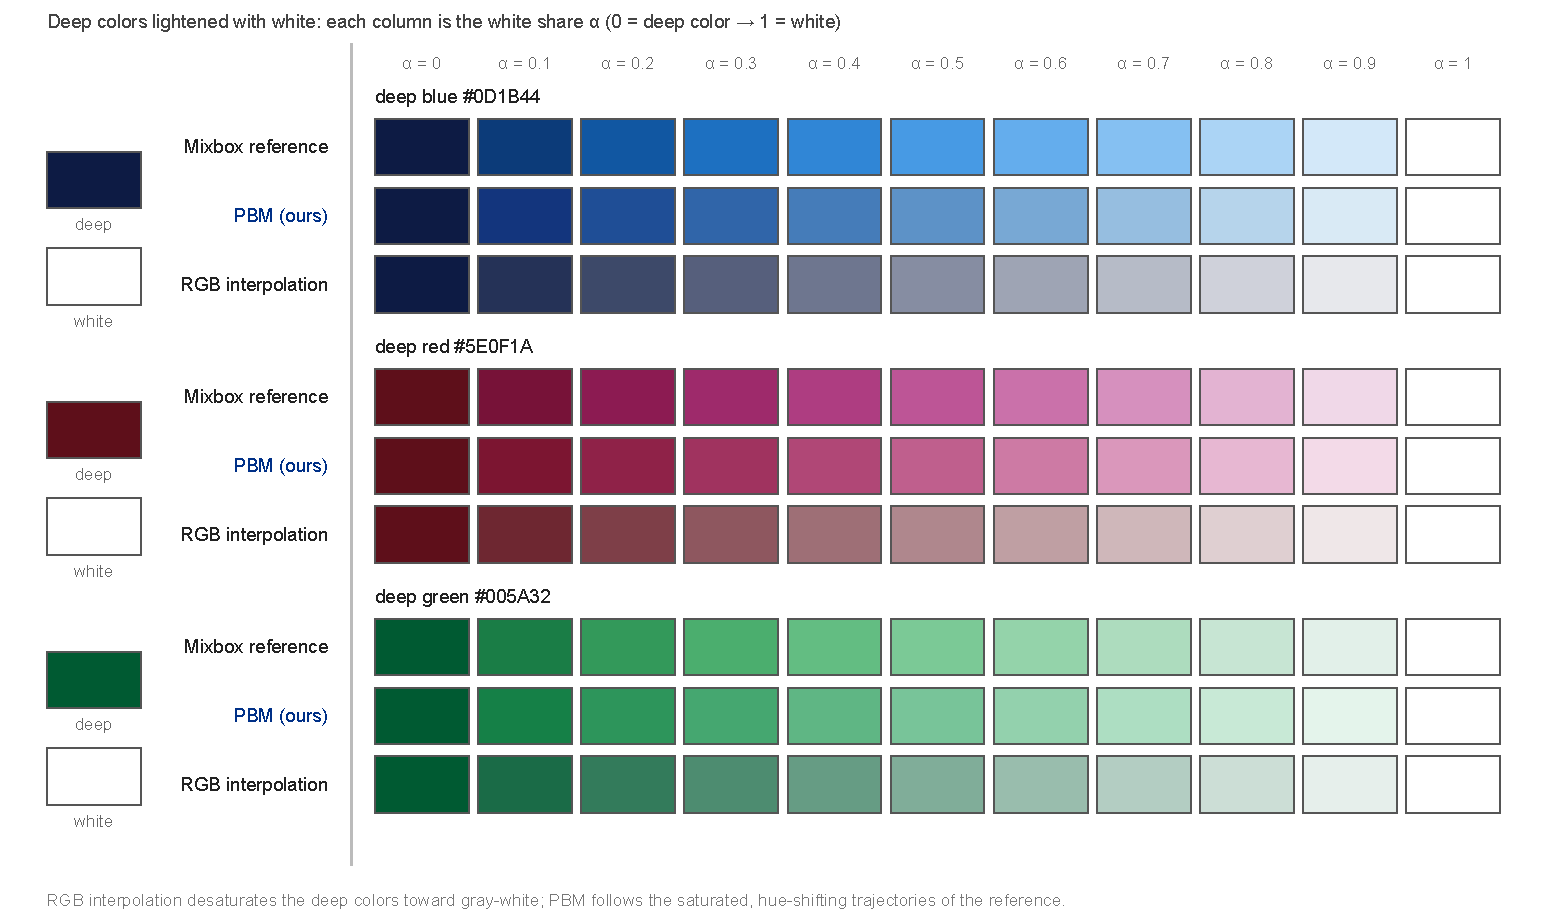
\includegraphics[width=\linewidth]{fig7-mixing-white.pdf}
\caption{Deep colors lightened with white. Each column is the white share $\alpha$ ($0$ = deep color, $1$ = white). RGB interpolation desaturates toward gray-white; PBM follows the chromatic, hue-shifting trajectories of the reference.}
\label{fig:white}
\end{figure}

\begin{figure}[t]
\centering
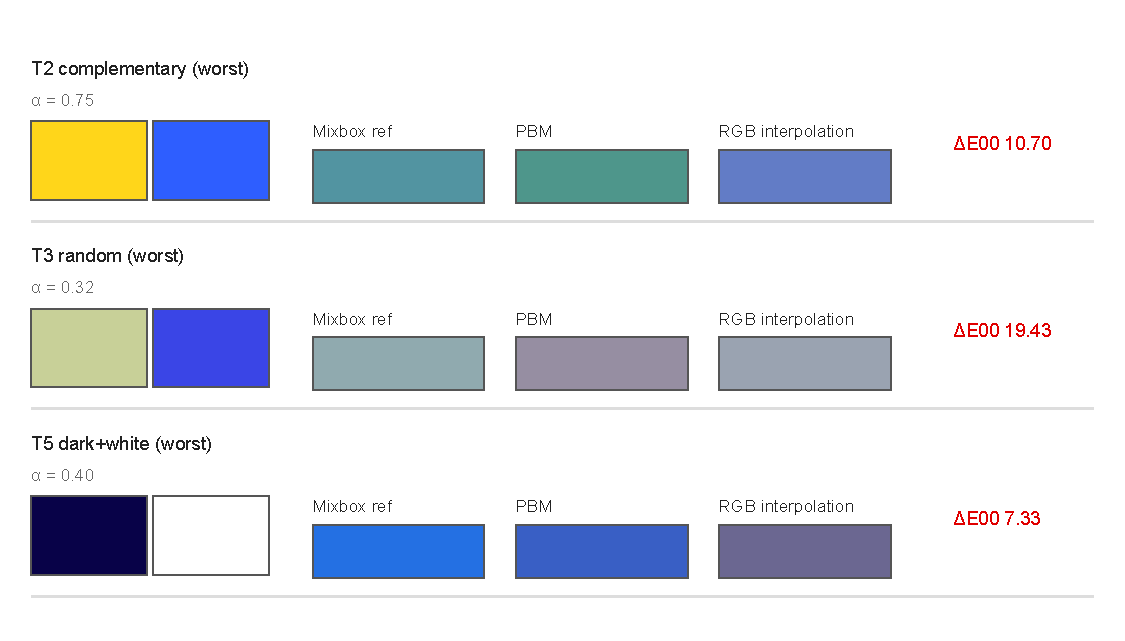
\includegraphics[width=0.82\linewidth]{fig5-worst-pairs.pdf}
\caption{Worst pairs of the T2 complementary, T3 random, and T5 dark-plus-white suites: inputs, Mixbox reference output, PBM output, RGB interpolation output, and $\Delta E_{00}$.}
\label{fig:worst}
\end{figure}

\subsection{Continuity and Exchange Symmetry}
\label{sec:continuity}

The continuity probe perturbs each channel of each input by $\pm1/255$ and the ratio by $+0.004$ for 4000 random pairs and records the largest change in the output $\Delta E_{00}$. The maximum single-step change is 1.388, with zero exceedances of 1.53. The chroma attenuation is necessary for this result: with $\mathrm{cSat}\equiv1$ the same probe measures 2.531 with 14 exceedances, because the ratio features have large gradients near the achromatic axis. \Cref{fig:continuity} shows the response for one deep-blue/white mix.

Exchange symmetry was measured on 5000 random pairs with seed 20260808. The maximum RGB difference between $F(\cb,\ct,\alpha)$ and $F(\ct,\cb,1-\alpha)$ is $6.7\times10^{-16}$, i.e.\ floating-point rounding from the different multiplication order in the two branches.

\begin{figure}[t]
\centering
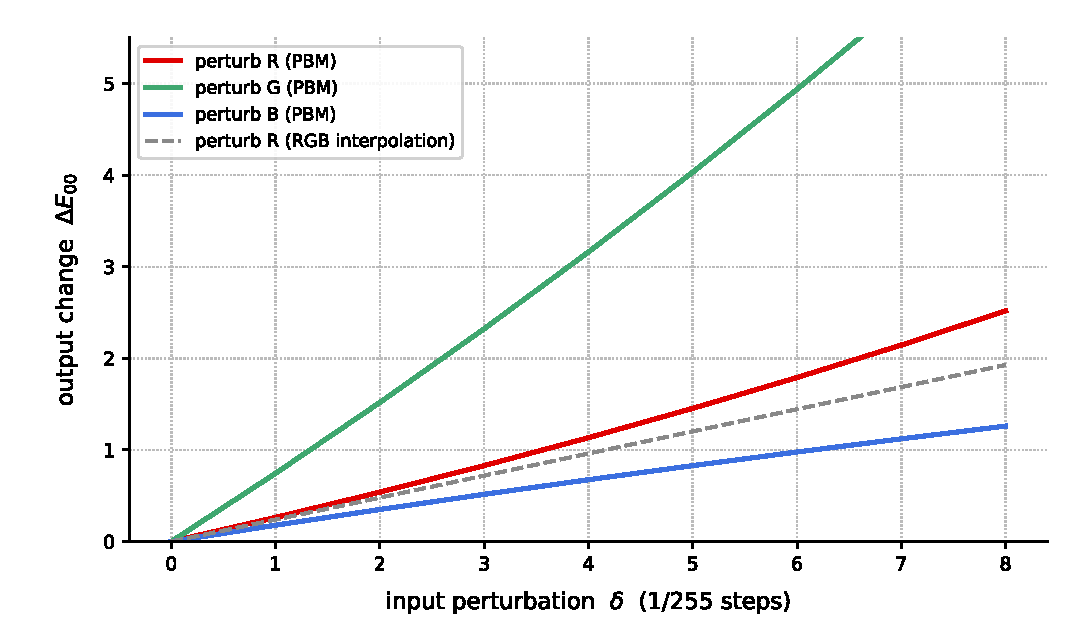
\includegraphics[width=0.72\linewidth]{fig6-continuity.pdf}
\caption{Neighborhood continuity: output change $\Delta E_{00}$ versus the input perturbation (1/255 steps on each channel of the deep blue $\#0D1B44$, mixed with white at $\alpha=0.5$); the dashed line shows the RGB interpolation response.}
\label{fig:continuity}
\end{figure}

\subsection{Runtime}
\label{sec:runtime}

\Cref{tab:runtime} reports per-mix timings measured in Node.js 26.13.1 on an AMD Ryzen~5 5600X under Windows~11. All models are loaded in the host V8 context: running the same code inside a \texttt{node:vm} sandbox inflates elementary-function calls (\texttt{Math.sqrt}, \texttt{Math.pow}) by one to two orders of magnitude---measured $8.9\times$ for PBM and $8.7\times$ for the reference---and would distort the comparison against the arithmetic-only baseline. PBM, Mixbox, and RGB interpolation use $10^{5}$ deterministic pairs and the best of nine repetitions after warm-up; the spectral K--M paths use a 50-pair subset because the iterative inversion dominates their runtime. Absolute timings are machine- and implementation-dependent; the ratios within this table are measured in one environment and are reported to support the interface argument, not as a general performance claim.

\begin{table}[t]
\centering
\small
\caption{Runtime cost per mix (best of nine repetitions after warm-up). The last column is the model's time relative to PBM.}
\label{tab:runtime}
\begin{tabular}{llrrr}
\toprule
Model & Path & ns/op & ops/s & Relative time \\
\midrule
PBM & analytic float arithmetic & 226 & 4{,}431,819 & 1.00 \\
Mixbox 2.0 & $256^{3}$ LUT lookup & 166 & 6{,}021,376 & 0.73 \\
RGB interpolation & linear blend & 16 & 63{,}572{,}791 & 0.070 \\
K--M spectral, direct & per-wavelength K/S $+$ D65$\times$CMF & 1{,}195 & 836,820 & 5.3 \\
K--M spectral, RGB-in & iterative unmix $+$ spectral mix & 22{,}400{,}000 & 45 & $9.9\times10^{4}$ \\
\bottomrule
\end{tabular}
\end{table}

PBM costs about 0.23 $\mu$s per mix, 1.4 times the reference's table lookup and 14 times a linear blend. The spectral K--M forward pipeline is not slow in itself: with pigment spectra known, the per-wavelength integration costs about 1.2 $\mu$s, roughly 5 times PBM. The obstacle is the interface: mixing two arbitrary RGB colors requires inverting each color into pigment concentrations, an iterative optimization costing about 22 ms per mix, or roughly $10^{5}$ times PBM. PBM's advantage is therefore not raw speed but the absence of a spectral representation, an inversion, or a multi-megabyte table. In interactive painting, mixing is applied per stroke or per operation rather than per rendered pixel; for per-pixel rendering, both models would be vectorized or implemented on the GPU, for which the analytic form is more portable. The absence of trigonometric and logarithmic evaluation in the harmonic correction also makes the model cheap to vectorize.

\subsection{Validation Against an Independent Synthetic Spectral World}
\label{sec:synthetic}

The evaluation above measures PBM against the reference. This section cross-validates against a ground truth computed from synthetic pigment spectra that were not used to fit PBM.

\paragraph{Dataset.}
The dataset contains 29 pigments: 24 functional hues covering the hue circle and the neutral scale, and 5 darkened derivations for the dark-plus-white suites. Each pigment is represented by separate absorption and scattering coefficients on a 10 nm grid over 380--750 nm (38 samples):
\begin{equation}
K(\lambda)=\kappa_{\mathrm{base}}+\sum_{i}A_{i}e^{-((\lambda-\mu_{i})/\sigma_{i})^{2}}
+\sum_{j}\frac{B_{j}}{1+e^{\pm((\lambda-\lambda_{j})/w_{j})}},
\qquad S(\lambda)=S_{\mathrm{base}}.
\label{eq:synthetic}
\end{equation}
Band positions are fixed by first-principles pigment chemistry (steep blue--green absorption edges for yellow/orange/red families, red-side rising edges for blue/green, a green-region band for magenta, and characteristic transition-metal or organic bands), whereas amplitudes, widths, bases, and scattering are calibrated to the publicly available BabelColor X-Rite ColorChecker Classic Avg30 spectra \cite{pascale2012} by coordinate descent (fit $\Delta E_{00}\le1.2$, most patches $\le0.2$). The ColorChecker patches are formulated color-card spectra, not pure-pigment masstone spectra; the K--M equations are closed for any reflectance spectrum, and the chart is designed for RGB displays, so no display calibration is required. The synthetic world is an approximation, not measured paint.

\paragraph{Pipeline and suites.}
The forward pipeline applies separate Duncan superposition of $K$ and $S$, evaluates \cref{eq:km} per wavelength, integrates against D65 and the CIE 1931 $2^{\circ}$ observer on the 10 nm grid, and converts to sRGB (clamping and flagging out-of-gamut samples). The inputs to all compared models are the rendered sRGB colors of the pure pigments, which avoids the issue of colors that cannot be mixed from pigments. Six suites mirror the T-suite structure: P1 (all 828 pairs of the 24-hue palette), P2 (9 stress pairs), P3 (2000 random pigment pairs, fresh seed 20260813), P5 (15 deep pigments $\times$ white), P5-buff (the same deep set $\times$ buff), and P5E (the two-sided tail grid). Out-of-gamut samples are clamped and counted.

\Cref{tab:synthetic} reports the results and \cref{fig:physical} visualizes three representative pairs.

\begin{table}[t]
\centering
\footnotesize
\setlength{\tabcolsep}{3pt}
\caption{$\Delta E_{00}$ against the synthetic-spectra reference (mean / max; bootstrap 95\% CI for random-set means in the note; out-of-gamut samples clamped and counted).}
\label{tab:synthetic}
\begin{tabular}{lcccccc}
\toprule
Model & P1 & P2 & P3 & P5 & P5-buff & P5E \\
 & {\scriptsize$n{=}828$, oog 6} & {\scriptsize$n{=}27$} & {\scriptsize$n{=}2000$, oog 35} & {\scriptsize$n{=}135$} & {\scriptsize$n{=}135$, oog 2} & {\scriptsize$n{=}150$, oog 6} \\
\midrule
PBM & 6.70 / 36.3 & 13.38 / 29.7 & 5.60 / 35.9 & 8.44 / 22.3 & 4.99 / 17.1 & 3.40 / 13.9 \\
Mixbox 2.0 & 6.46 / 31.5 & 12.71 / 24.9 & 5.10 / 30.2 & 8.86 / 25.0 & 4.56 / 18.9 & 3.39 / 20.9 \\
RGB interpolation & 6.14 / 29.5 & 11.25 / 20.4 & 4.89 / 25.4 & 8.24 / 27.0 & 5.95 / 15.8 & 3.88 / 26.9 \\
K--M display-value & 5.55 / 30.5 & 8.82 / 16.6 & 4.38 / 30.5 & 12.13 / 30.8 & 4.95 / 18.1 & 4.25 / 28.2 \\
\bottomrule
\end{tabular}

\smallskip
{\scriptsize Bootstrap 95\% CI (mean): PBM P1 [6.320, 7.045], P3 [5.390, 5.822], P5 [7.610, 9.258]; Mixbox P1 [6.080, 6.808], P3 [4.884, 5.333], P5 [7.964, 9.786].}
\end{table}

\begin{figure}[t]
\centering
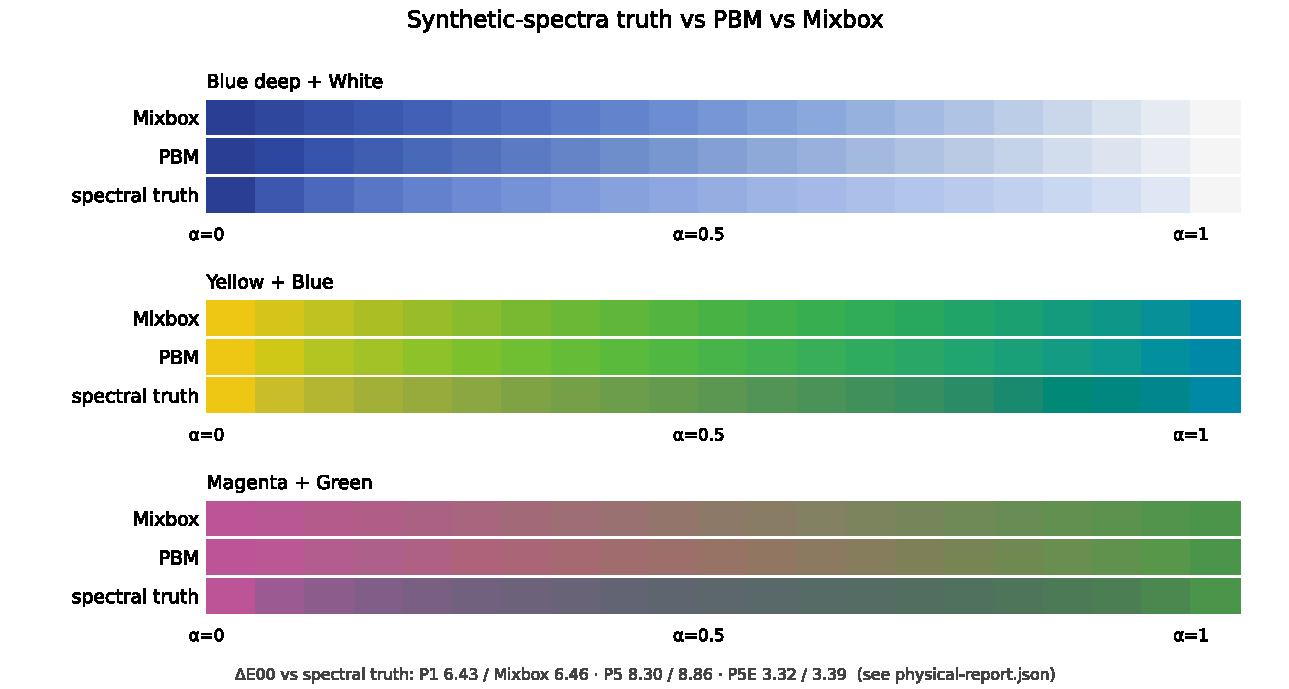
\includegraphics[width=0.88\linewidth]{fig8-physical.pdf}
\caption{Synthetic-spectra truth versus PBM and Mixbox for three representative pigment pairs (deep blue $\times$ white, yellow $\times$ blue, magenta $\times$ green) over $\alpha=0$--$1$ (21 steps).}
\label{fig:physical}
\end{figure}

Three observations follow. First, PBM and the reference are comparable on this world: the per-suite mean differences $\mathrm{PBM}-\mathrm{Mixbox}$ range from $-0.42$ (P5) to $+0.67$ (P2), and every pair of bootstrap intervals overlaps. Neither model was trained on this world, so the parity is evidence that PBM's accuracy is not an artifact of fitting the reference's outputs. PBM is closer on P5 and P5E; the reference is closer on P1, P2, P3, and P5-buff; we did not test the differences for significance. Second, the hue trajectories agree: \cref{tab:hue} reports mean and median absolute hue differences for chromatic samples ($C^{\ast}>10$). PBM's mean hue error is lower on three of the six suites (P5, P5-buff, P5E) and within $2^{\circ}$ on the others. Third, the residual per-suite mean errors (3.40--13.38 $\Delta E_{00}$) are structural: the synthetic world mixes by spectral K--M, whereas Mixbox mixes in a trained latent polynomial.

\begin{table}[t]
\centering
\small
\caption{Hue agreement with the synthetic spectral truth: mean and median absolute hue difference in degrees over chromatic samples ($C^{\ast}>10$).}
\label{tab:hue}
\begin{tabular}{lcc}
\toprule
Suite & PBM & Mixbox 2.0 \\
\midrule
P1 & 11.33 / 6.62 & 11.01 / 5.96 \\
P2 & 23.17 / 17.23 & 21.46 / 18.01 \\
P3 & 9.27 / 4.62 & 8.64 / 3.73 \\
P5 & 9.54 / 5.77 & 9.67 / 7.15 \\
P5-buff & 8.59 / 5.79 & 8.62 / 5.30 \\
P5E & 2.56 / 0.62 & 2.73 / 0.74 \\
\bottomrule
\end{tabular}
\end{table}

\paragraph{What this establishes and what it does not.}
The experiment supports two claims: (i) PBM's accuracy is not an artifact of overfitting the reference's outputs, because it matches the reference against an independent synthetic spectral world; and (ii) the qualitative behavior families---yellow $\times$ blue gives green, complementary pairs give muted colors, deep $+$ white preserves hue---also hold under two-constant spectral K--M mixing. It does not establish that PBM predicts real-paint masstone mixing, nor that it is closer to real paint than the reference. The synthetic world is itself an approximation, and PBM's relation to real paint is bounded by the reference's relation to real paint plus PBM's measured deviation from the reference.

\subsection{Threats to Validity}
\label{sec:threats}

\paragraph{Reference dependence.}
PBM is fitted to Mixbox~2.0. If the reference changes, the constants must be re-estimated with the procedure of \cref{sec:estimation}. The measured accuracy is relative to that reference; it does not bound the error against measured paint samples.

\paragraph{Synthetic world.}
The cross-validation uses two-constant K--M mixing of synthetic spectra calibrated to ColorChecker patches. Both the two-constant approximation and the patch-based calibration limit the interpretation; the synthetic world is not a substitute for measured pigment spectra.

\paragraph{Metric.}
We use CIEDE2000 with uniform weights. Other color-difference formulas or observer/illuminant choices may reorder individual pairs and change the reported means.

\paragraph{Sampling.}
Fixed suites are in-sample; only the random sets have confidence intervals. The CIs cover sampling variability of the mean, not model-selection or implementation uncertainty.

\paragraph{Scope.}
The model is defined for opaque, uniformly mixed colors in sRGB display space. It does not model layering, glazing, opacity, texture, or spectral output.

\section{Limitations and Future Work}
\label{sec:limitations}

\paragraph{Nature of the residual error.}
The largest T5 residual (near-black purple, $\Delta E_{00}\approx5.8$) and the largest main-suite residuals (lightness-gap and hue-opposition pairs, 10.7--23.8) share an origin: the reference expresses its gamut on a four-pigment basis, and the high-order cross-channel correlations of red-family and violet pigments are properties of that latent representation, not of per-channel independent forms. PBM approaches the latent behavior along four dimensions---the K--M core, the power-law exponents, the harmonic correction, and the $\varphi$ map---but the remaining errors dominate the maximum statistics.

\paragraph{Near-neutral deep blind zone.}
Near-neutral deep colors ($\mathrm{maxd}\in[0.02,0.06]$) fall below the gate and are mixed by the core alone. The power-law staircase was fitted on chromatic deep colors, whose channel structure differs from the approximately uniform exponent needed for grayish deep colors. The residual measures a maximum of 9.5 $\Delta E_{00}$ on the light side and a mean of 2.441 over T5E. This is inside the design targets but is the largest maximum among the dark-plus-white design-target suites (T5, T5E, and tail). The $\varphi$ map reduced but did not eliminate it.

\paragraph{Relation to Mixbox.}
Mixbox applies linear latent mixing followed by a polynomial latent mapping and was trained on measured pigment spectra. PBM applies an analytic K--M structure and an analytic repair layer fitted to the reference's output. Because the reference's latent space is trained on measured pigment data, PBM inherits part of the reference's physical plausibility transitively; its error against real paint is bounded by the reference's own error plus PBM's measured deviation from the reference. That deviation is the price of a fully analytic model that can be implemented without trained tables or license restrictions.

\paragraph{Remaining limitations.}
\begin{enumerate}
\item The per-channel independent structure cannot represent the reference's high-order cross-channel correlations; this is the source of the largest errors.
\item The constants are fitted to Mixbox~2.0. If the reference changes, the constants must be re-estimated with the procedure of \cref{sec:estimation}; they do not transfer to a different reference.
\item The linear directional response cannot reconcile magenta and deep red under one univariate form. The magenta members of T5 measure means of 1.91--1.99 and maxima of 2.19--2.86, with the near-black purple $\#2A0A5E$ at a mean of 3.93 and a maximum of 5.82, and the dark violet $\#080248$ at 5.14 / 7.33.
\item The harmonic correction is linear over a hand-designed feature template. Its residual is largest for pairs whose reference trajectories are non-monotone in the mixing ratio. A non-linear but still analytic correction, and additional latent channels on the model side, are left for future work.
\item The synthetic-spectra validation confirms model parity and qualitative family behavior against an independent two-constant K--M world. A measured counterpart would require an authorized release of measured paint spectra.
\end{enumerate}

Future work includes extending the feature structure beyond the current template, re-fitting the staircase for the near-neutral blind zone, adding residual (non-spectral) latent channels to the core, generalizing the model to layered compositing, and re-fitting against physical paint measurements when such data are available.

\section{Conclusion}
\label{sec:conclusion}

We described PBM, a reference-calibrated analytic model for pigment mixing in sRGB display-value space. The model combines a K--M/Duncan-structured core with a repair layer of three continuously blended mechanisms: a per-channel power-law target for dark-plus-light mixtures, an additive harmonic correction for complementary pairs, and a soft role assignment that makes the model exchange-symmetric. The harmonic correction is linear over a seventeen-feature ratio template, so the model contains no trigonometric or logarithmic evaluation; only arithmetic, powers, and square roots remain. It is $O(1)$ and table-free, returns its inputs exactly at $\alpha=0$ and $\alpha=1$, is continuous by construction, and is exchange-symmetric up to floating-point rounding ($6.7\times10^{-16}$ in the reported probe). The 51 harmonic coefficients are obtained in closed form by least squares, and the remaining 14 scalars by coordinate descent on the same loss; all constants are reproduced identically in four language ports.

Against Mixbox~2.0, PBM measures a mean $\Delta E_{00}$ of 2.258 (maximum 7.3) on the dark-plus-white suite, 2.377 on held-out dark-plus-white pairs, and 2.719--2.852 on held-out random pairs, consistently below RGB interpolation and raw K--M superposition. Against an independent synthetic spectral world, its per-suite mean errors differ from the reference's by at most 0.67 $\Delta E_{00}$, with all bootstrap intervals overlapping, and its mean hue error is lower on three of six suites. The remaining large errors (10.7--23.8 $\Delta E_{00}$) concentrate in pairs that combine a large lightness gap with hue opposition, where per-channel independent forms cannot follow the reference's cross-channel correlations, and in the near-neutral deep blind zone.

The practical value of the model is what it does not require: no spectral data, no lookup tables, no trained latent mapping, and no third-party licensed component. It can therefore replace linear RGB interpolation in painting software, game engines, and web applications that cannot accommodate a table-based reference, while reproducing the qualitative behavior of pigment mixing---blue and yellow produce green, complementary pairs produce muted neutrals, and deep colors remain chromatic when lightened with white. The evaluation reported here bounds that claim to agreement with the reference and with a synthetic spectral world; it does not establish agreement with measured paint.


\begin{thebibliography}{99}
\bibitem{kubelka1931} P.~Kubelka and F.~Munk. Ein Beitrag zur Optik der Farbanstriche. \emph{Zeitschrift f\"ur Technische Physik}, 12:593--601, 1931.
\bibitem{duncan1940} D.~R. Duncan. The colour of pigment mixtures. \emph{Proceedings of the Physical Society}, 52:390--400, 1940.
\bibitem{saunderson1942} J.~L. Saunderson. Calculation of the color of pigmented plastics. \emph{Journal of the Optical Society of America}, 32:727--736, 1942.
\bibitem{pointer1980} M.~R. Pointer. The gamut of real surface colours. \emph{Color Research \& Application}, 5(3):145--155, 1980.
\bibitem{haase1992} C.~S. Haase and G.~W. Meyer. Modeling pigmented materials for realistic image synthesis. \emph{ACM Transactions on Graphics}, 11(4):305--335, 1992.
\bibitem{gossett2004} N.~Gossett and B.~Chen. Paint inspired color mixing and compositing for visualization. In \emph{Proceedings of IEEE InfoVis}, pages 113--118, 2004.
\bibitem{sharma2005} G.~Sharma, W.~Wu, and E.~N. Dalal. The CIEDE2000 color-difference formula: implementation notes, supplementary test data, and mathematical observations. \emph{Color Research \& Application}, 30(1):21--30, 2005.
\bibitem{lu2014} J.~Lu, S.~DiVerdi, W.~Chen, C.~Barnes, and A.~Finkelstein. RealPigment: paint compositing by example. In \emph{Proceedings of NPAR}, pages 21--30, 2014.
\bibitem{simonot2014} L.~Simonot and M.~H\'ebert. Between additive and subtractive color mixings: intermediate mixing models. \emph{Journal of the Optical Society of America A}, 31(1):58--66, 2014.
\bibitem{aharoni2017} E.~Aharoni-Mack, Y.~Shambik, and D.~Lischinski. Pigment-based recolorings of watercolor paintings. In \emph{Proceedings of NPAR}, Article~1, 2017.
\bibitem{tan2019} J.~Tan, S.~DiVerdi, J.~Lu, and Y.~Gingold. Pigmento: pigment-based image analysis and editing. \emph{IEEE Transactions on Visualization and Computer Graphics}, 25(9), 2019.
\bibitem{shugrina2020} M.~Shugrina, A.~Kar, S.~Fidler, and K.~Singh. Nonlinear color triads for approximation, learning and direct manipulation of color distributions. \emph{ACM Transactions on Graphics}, 39(4), Article~97, 2020.
\bibitem{sochorova2021} \v{S}.~Sochorov\'a and O.~Jamri\v{s}ka. Practical pigment mixing for digital painting. \emph{ACM Transactions on Graphics}, 40(6), Article~234, 2021.
\bibitem{wyszecki2000} G.~Wyszecki and W.~S. Stiles. \emph{Color Science: Concepts and Methods, Quantitative Data and Formulae}. 2nd edition, John Wiley \& Sons, 2000.
\bibitem{pascale2012} D.~Pascale. The ColorChecker pages: ColorChecker data (averaged spectral measurements of 30 charts). BabelColor, 2012. \url{http://www.babelcolor.com/colorchecker-2.htm}.
\end{thebibliography}

\crefalias{section}{appendix}
\appendix

\section{Evaluation Suite Specification}
\label{app:suite}

\subsection{Reference and Metric}
\begin{itemize}
\item Reference: Mixbox~2.0 \texttt{lerpFloat(base, tint, a)}, loaded from the official distribution; research comparison only, not part of the algorithm.
\item Only the float path is used (sRGB display values in $[0,1]$), avoiding 8-bit quantization.
\item Metric: CIEDE2000 with $k_{L}=k_{C}=k_{H}=1$, including the $G$ factor, hue-angle wrap, weighting functions $S_{L},S_{C},S_{H}$, and the rotation term $R_{T}$.
\item Replication check: the implementation is validated against the 34 reference pairs of Sharma et al.\ the maximum deviation is $4.95\times10^{-5}$.
\item Confidence intervals: bootstrap 95\% percentile intervals (1000 resamples) with a fixed resampling stream.
\end{itemize}

\subsection{Test Sets}
\begin{itemize}
\item T1: all pairs of the preset palette (10 bases $\times$ 8 tints) at $\alpha\in\{0.25,0.5,0.75\}$ (240 samples).
\item T2: 19 stress pairs at three ratios (57 samples), listed in \cref{tab:t2}.
\item T3: uniform random sRGB pairs with uniform $\alpha$, seed 20260808, $n=2000$ (configurable).
\item T4: 10 colors at $\alpha\in\{0,1\}$ with self-mixing; channel tolerance 0.01.
\item T5: 20 fixed deep colors and 24 random deep colors, each at $\alpha\in\{0.1,0.2,\dots,0.9\}$ (396 samples).
\item T5-heldout: 24 random deep colors from seed 20260812 at the same $\alpha$ grid (216 samples).
\item tail: 20 T5 fixed colors at $\alpha\in\{0.92,0.93,\dots,0.99\}$ (160) and 9 blind-spot colors at the T5 $\alpha$ grid (81).
\item T5E: 20 T5 fixed colors at deep-side $\alpha$ (120), 12 near-neutral colors at deep-side $\alpha$ (72), and the same 12 at light-side $\alpha$ (48).
\end{itemize}

\begin{table}[t]
\centering
\footnotesize
\setlength{\tabcolsep}{3pt}
\caption{T2 stress pairs.}
\label{tab:t2}
\begin{tabular}{p{0.16\linewidth}p{0.78\linewidth}}
\toprule
Category & Pairs \\
\midrule
complementary (3) & \#E8321F + \#00D5C0; \#FFD61A + \#2E5EFF; \#E33BA8 + \#00B359 \\
RYB mismatch (6) & \#E8321F + \#00B359; \#2E5EFF + \#FF7A1A; \#E8321F + \#2E5EFF; \#FFD61A + \#00B359; \#FFD61A + \#00D5C0; \#E33BA8 + \#00D5C0 \\
white/black (6) & \#E8321F, \#2E5EFF, \#FFD61A, each $\times$ \{\#FFFFFF, \#000000\} \\
similar (4) & \#E8321F + \#FF7A1A; \#FFD61A + \#FF7A1A; \#2E5EFF + \#8A5BE0; \#00B359 + \#00D5C0 \\
\bottomrule
\end{tabular}
\end{table}

\subsection{The T5 and T5E Suites}
\label{app:t5}

\paragraph{T5 fixed colors.}
\Cref{tab:t5colors} lists the 20 fixed colors: 10 pain-point colors and 10 family extensions. The random deep colors are rejection-sampled until $\max(\mathbf{c})\in[0.30,0.60]$, $\min(\mathbf{c})\le0.08$, and $\max(\mathbf{c})-\min(\mathbf{c})\ge0.25$; T5 uses seed 20260810 and T5-heldout seed 20260812.

\begin{table}[t]
\centering
\small
\caption{T5 fixed deep colors (sRGB hex and display-value floats).}
\label{tab:t5colors}
\begin{tabular}{llll}
\toprule
Hex & Float RGB & Hex & Float RGB \\
\midrule
$\#0D1B44$ & 0.051, 0.106, 0.267 & $\#0A2A6E$ & 0.039, 0.165, 0.431 \\
$\#000080$ & 0.000, 0.000, 0.502 & $\#8E1F0A$ & 0.557, 0.122, 0.039 \\
$\#001B75$ & 0.000, 0.106, 0.459 & $\#005A32$ & 0.000, 0.353, 0.196 \\
$\#001E80$ & 0.000, 0.118, 0.502 & $\#00552B$ & 0.000, 0.333, 0.169 \\
$\#080248$ & 0.031, 0.008, 0.282 & $\#00585E$ & 0.000, 0.345, 0.369 \\
$\#5F1708$ & 0.373, 0.090, 0.031 & $\#2A0A5E$ & 0.165, 0.039, 0.369 \\
$\#5E0F1A$ & 0.369, 0.059, 0.102 & $\#4A0B6E$ & 0.290, 0.043, 0.431 \\
$\#4A3A05$ & 0.290, 0.227, 0.020 & $\#6E0B4A$ & 0.431, 0.043, 0.290 \\
$\#280501$ & 0.157, 0.020, 0.004 & $\#7A3B00$ & 0.478, 0.231, 0.000 \\
$\#250903$ & 0.145, 0.035, 0.012 & $\#6E4A00$ & 0.431, 0.290, 0.000 \\
\bottomrule
\end{tabular}
\end{table}

\paragraph{T5E.}
Deep-side $\alpha$ levels are 0.001, 0.005, 0.01, 0.02, 0.05, and 0.1; light-side levels are 0.92, 0.95, 0.98, and 0.99. The near-neutral group is \#000B2E, \#06052E, \#1A0F22, and \#0A1A18, plus 8 random colors from seed 20260816, rejection-sampled with $\max\in[0.04,0.10]$ and chroma range $\in[0.02,0.06]$.

\paragraph{Tail blind-spot colors.}
$\#0D1B44$, $\#001B75$, $\#000080$, $\#001E80$, $\#080248$, $\#0A2A6E$, $\#2A0A5E$, $\#060538$, $\#000333$.

\subsection{Split and Statistics}
\begin{itemize}
\item Fitting draw: T1, T2, T5, T5E, tail, the first 800 pairs of T3 (seed 20260808), 6000 pseudo-random pairs (seed 999), and 12 anchored complementary pairs at 19 ratios each.
\item Held-out: T3 pairs 800--1999 of the same draw, T3 draws with seeds 20260809 and 20260811, and T5-heldout (seed 20260812).
\item For each model and set we report mean, maximum, median, 95th percentile, standard deviation, and (for random sets) a bootstrap 95\% interval on the mean.
\item Reported figures are generated from the reference implementation by the repository tooling; the seed of every draw is stated in the caption or in this appendix.
\end{itemize}

\section{Harmonic Correction Coefficients}
\label{app:coeff}

The 51 coefficients of \cref{eq:gamma} are listed below in feature order (\cref{tab:features}: intercept, \texttt{lum}, \texttt{dgug}, \texttt{dcmucm}, \texttt{wUcP}, \texttt{u2}, \texttt{pm}, \texttt{dg}, \texttt{op}, \texttt{span}, \texttt{drur}, \texttt{pn}, \texttt{Mmn}, \texttt{lumU}, \texttt{ur}, \texttt{dcAbs}, \texttt{gRu}); the intercept is first.

\paragraph{R channel (17 coefficients).}
$-0.24945965$, $-0.00458899$, $0.00415136$, $-0.03758060$, $0.05450570$, $0.09989345$, $0.25226195$, $0.02321094$, $0.15029394$, $0.03230901$, $0.03005819$, $0.34621807$, $-0.57046216$, $-0.00274566$, $0.03208997$, $-0.05313629$, $-0.02941071$.

\paragraph{G channel (17 coefficients).}
$-0.15650537$, $0.14061150$, $-0.03620353$, $0.03735064$, $0.02174583$, $0.02381613$, $-0.06481304$, $-0.02027288$, $0.13851721$, $0.13327492$, $0.01269829$, $0.03768178$, $-0.05558582$, $0.03768944$, $0.01505410$, $0.02180116$, $-0.01767582$.

\paragraph{B channel (17 coefficients).}
$0.16757082$, $-0.04373748$, $0.02221282$, $-0.02131140$, $-0.08893948$, $0.05973609$, $-0.09324463$, $-0.00242072$, $-0.11889782$, $-0.08066689$, $-0.01881345$, $-0.40457567$, $0.51586855$, $-0.01855359$, $0.03390971$, $-0.01807147$, $-0.04148750$.

\section{Synthetic Spectral Dataset}
\label{app:synthetic}

\subsection{Dataset}
The model is two-constant K--M with separate absorption and scattering per pigment on a 10 nm grid over 380--750 nm (38 samples):
\begin{equation}
K(\lambda)=\kappa_{\mathrm{base}}+\sum_{i}A_{i}e^{-((\lambda-\mu_{i})/\sigma_{i})^{2}}+\sum_{j}\frac{B_{j}}{1+e^{\pm((\lambda-\lambda_{j})/w_{j})}},
\qquad S(\lambda)=S_{\mathrm{base}}.
\end{equation}
Every parameter is a fixed constant; the dataset is reproduced deterministically by the tooling. Band positions follow first-principles pigment chemistry: yellow, orange, red, and earth families carry steep logistic absorption edges in the blue--green region ($\lambda_{0}\approx490$--$585$ nm), blue and green carry red-side rising edges ($\approx610$--$660$ nm), magenta and purple carry Gaussian bands in the green region ($\approx550$--$580$ nm), and transition-metal or organic pigments add characteristic bands ($\approx430$--$660$ nm). Amplitudes, widths, bases, and scattering are calibrated to the BabelColor X-Rite ColorChecker Classic Avg30 spectra \cite{pascale2012} by coordinate descent (fit $\Delta E_{00}\le1.2$, most patches $\le0.2$). The patches are formulated color-card spectra rather than pure-pigment masstone spectra; the K--M equations are closed for any reflectance spectrum, and the chart is designed for RGB displays, so no display calibration is required.

The dataset contains 29 pigments: 24 functional hues (white, black, buff, gray light/mid/dark, gray blue, two yellows, two oranges, two reds, two magentas, purple, three blues, cyan, two greens, two earths) and 5 deep derivations (deep blue, red, green, magenta, purple) for the P5 suites. No third-party measurement data are contained in the repository; the numerical parameters are fitted offline to the documented public source and the fitted values are published.

\subsection{Forward Pipeline and Validation}
The forward pipeline applies separate Duncan superposition $K=(1-\alpha)K_{A}+\alpha K_{B}$ and $S=(1-\alpha)S_{A}+\alpha S_{B}$, evaluates $\kappa=K/S$ and \cref{eq:km}, integrates against D65 and the CIE 1931 $2^{\circ}$ observer on the 10 nm grid (trapezoidal rule, normalized to $Y=100$), and converts to IEC 61966-2-1 sRGB with clamping and out-of-gamut flagging.

The dataset is self-checked by the tooling: all 29 pigments satisfy $\Rinf\in(0,1)$ and $K\ge0$, $S>0$; unmix reconstruction of the pure primaries has $\Delta E_{00}=0.000$; spectral mixing is identity at $\alpha=0,1$; yellow $\times$ blue renders green ($h^{\circ}\in(110,190)$); magenta $\times$ green and red $\times$ cyan render muted colors ($C^{\ast}<30$ and $<40$); deep $+$ white preserves hue ($|\Delta h|<40^{\circ}$ over $\alpha=0.25$--$0.75$); and every pigment renders inside its family hue window. Saturated pure pigments can legitimately exceed the sRGB gamut; such samples are flagged and clamped before model input (P1: 6/828; P3: 35/2000; P5: 0/135).

\subsection{Suites}
\begin{itemize}
\item P1: all $\binom{24}{2}$ pairs of the 24-hue palette at $\alpha\in\{0.25,0.5,0.75\}$ (828 samples).
\item P2: nine complementary/stress pairs at the same ratios (27 samples).
\item P3: 2000 random pigment pairs with uniform $\alpha$, seed 20260813.
\item P5: 15 deep pigments $\times$ white at $\alpha\in\{0.1,\dots,0.9\}$ (135 samples).
\item P5-buff: the same deep set $\times$ buff at the same grid (135 samples).
\item P5E: the deep set $\times$ white at $\alpha\in\{0.001,0.005,0.01,0.02,0.05,0.1,0.92,0.95,0.98,0.99\}$ (150 samples).
\end{itemize}

\section{Inversion Measurements}
\label{app:inversion}

All numbers in this appendix were measured on the Mixbox~2.0 reference (float path).

\subsection{Inverted Power Exponent}
For anchored colors, the exponent is inverted per channel as in \cref{eq:inversion}. \Cref{tab:d1} reports the inverted exponent over $\alpha\in\{0.1,\dots,0.9\}$ for the absorption band of synthetic anchored colors (inverting the maximal channel). The drift is below 0.2 in every family; the breakdown at $\alpha\to1$ is the region addressed by the $\varphi$ map.

\begin{table}[t]
\centering
\small
\caption{Inverted exponent $p$ over $\alpha$ for the absorption band (measured).}
\label{tab:d1}
\begin{tabular}{lccccc}
\toprule
Family & $\alpha=0.1$ & $\alpha=0.3$ & $\alpha=0.5$ & $\alpha=0.7$ & $\alpha=0.9$ \\
\midrule
$B$ & 0.97 & 0.97 & 0.98 & 1.00 & 1.03 \\
$R$ & 0.98 & 1.00 & 1.04 & 1.09 & 1.16 \\
$G$ & 1.00 & 1.03 & 1.07 & 1.12 & 1.18 \\
\bottomrule
\end{tabular}
\end{table}

\Cref{tab:d2} is an excerpt of the anchor inversion table at $\alpha=0.5$, where $s$ is the position of the channel along the chroma direction. For the synthetic color $(0.01,v,0.01)$, the $s=1$ channel (G maximal) gives $v=0.05\rightarrow1.07$, $0.12\rightarrow1.06$, $0.25\rightarrow0.81$, $0.35\rightarrow0.58$, $0.55\rightarrow0.42$; the fast bright-end regime applies only for $v>0.25$.

\begin{table}[t]
\centering
\small
\caption{Anchor inversion table (excerpt, $\alpha=0.5$).}
\label{tab:d2}
\begin{tabular}{lccccc}
\toprule
Color & Ch & $v$ & $s$ & $p$ \\
\midrule
$\#0D1B44$ & R & 0.051 & 0.00 & 2.05 \\
$\#0D1B44$ & G & 0.106 & 0.26 & 0.84 \\
$\#0D1B44$ & B & 0.267 & 1.00 & 0.23 \\
$\#080248$ & R & 0.031 & 0.09 & 2.25 \\
$\#080248$ & B & 0.282 & 1.00 & 0.12 \\
$\#4A0B6E$ & B & 0.431 & 1.00 & 0.85 \\
$\#6E0B4A$ & G & 0.043 & 0.00 & 1.59 \\
$\#5F1708$ & R & 0.373 & 1.00 & 0.76 \\
$\#5F1708$ & G & 0.090 & 0.17 & 1.77 \\
$\#5F1708$ & B & 0.031 & 0.00 & 0.90 \\
$\#8E1F0A$ & R & 0.557 & 1.00 & 0.62 \\
$\#005A32$ & G & 0.353 & 1.00 & 0.57 \\
$\#005A32$ & B & 0.196 & 0.56 & 1.04 \\
$\#6E0B4A$ & B & 0.290 & 0.64 & 0.91 \\
\bottomrule
\end{tabular}
\end{table}

\subsection{Residuals and Coupling}
For $v=0$ channels, the reference curves are independent of the pigment and depend only on the channel (for example, both R and G of $\#000080$ are zero but their reference curves differ), which motivates the residual term. The residuals measured during fitting were approximately 1.85 (R), 1.0 (G), and 1.1 (B), and were fine-tuned with decay in the channel value.

The coupling term is measured by fixing $B=0.431$ and $G=0.043$ and sweeping $R$ at $\alpha=0.5$ (\cref{tab:d3}). The relation is a monotone S-shape: the purple $\#4A0B6E$ ($R=0.29$) has $p_{B}=0.85$, whereas pure blue ($R\approx0$) has $p_{B}=0.12$--$0.17$. The coupling is symmetric: high $B$ slows $R$ ($p_{R}$ rises from 1.04 to 2.02 as $B$ goes from 0 to 0.431).

\begin{table}[t]
\centering
\small
\caption{Channel coupling: inverted $p_{B}$ as a function of $R$ (measured).}
\label{tab:d3}
\begin{tabular}{lccccccc}
\toprule
$R$ & 0.03 & 0.06 & 0.10 & 0.15 & 0.20 & 0.25 & 0.30 \\
$p_{B}$ & 0.17 & 0.21 & 0.35 & 0.60 & 0.73 & 0.80 & 0.85 \\
\bottomrule
\end{tabular}
\end{table}

\subsection{Directional Responses}
Inverting the T5 red-dominant fixed colors per $\alpha$ preserves $\alpha$-constancy ($\sigma<0.1$); \cref{tab:d4} reports the per-channel need. Three structural signals appear: red-family G holding ($\#5E0F1A$ and $\#8E1F0A$ need $G\approx1.7$--$1.8$), yellow-brown B holding ($\#906D00$ needs $B\approx1.5$), and red transmission (the R need is 0.62--0.77). A least-squares fit over the inversion residuals of 11 red-dominant fixed colors, with the same linear form $\delta_{c}=a+k\,v$ for all three channels, yields the unified responses of \cref{eq:deltas}. The range gate $g_{R}\sigma_{8}(v_{R}-\mathrm{RTH})$ with $\mathrm{RTH}=0.21929798$ is necessary because the directional coefficients change sign below it.

\begin{table}[t]
\centering
\small
\caption{Red-family inversion: per-channel exponent need (measured).}
\label{tab:d4}
\begin{tabular}{lccc}
\toprule
Color & R need & G need & B need \\
\midrule
$\#5E0F1A$ deep red & 0.77 & 1.78 & 0.89 \\
$\#8E1F0A$ deep red & 0.62 & 1.71 & 0.88 \\
$\#906D00$ ochre & 0.72 & 0.95 & 1.49 \\
$\#940C7C$ magenta & 0.99 & 1.31 & 0.98 \\
\bottomrule
\end{tabular}
\end{table}

\subsection{Complementary Families}
Inverting the reference on complementary pairs reveals a family-structured residual: for each hue-opposition family the error concentrates in the middle of the mixing range with the shape $4a(1-a)$, and its amplitude is a smooth function of the two input colors. For example, the bright-yellow $\times$ deep-blue family has a G-channel error near zero, a B-channel error at most 0.05, and an R-channel error following $4a(1-a)$ with amplitude 0.28--0.29 for $\alpha\in[0.4,0.9]$. Because the reference's latent space is non-linear, the amplitudes vary smoothly across families and a single amplitude per family is insufficient; the harmonic correction is therefore a linear model over the seventeen-feature template, fitted on a corpus of complementary-family measurements (weighted by a factor of 10), with 17 coefficients per channel. The endpoint suppression $h(a)$ and the chroma attenuation $\mathrm{cSat}$ are structural rather than fitted.


\end{document}
